\documentclass[9pt]{beamer}
\usetheme{Madrid}
\usepackage{mathtools}
\usepackage{bm}
\usepackage{esvect}
\usepackage{amsmath}
\usepackage{physics}
\usepackage{empheq}
\usepackage[many]{tcolorbox}

%$\vv{\bm{L}}

\title{Majorana's Beach}
  
\author{J.J. G\'omez Cadenas}
 
\institute{Donostia International Physics Center (DIPC)} % (optional)
 
\date[November 22, 2021] % (optional)
{Caltech in Meta Space, 22 November 2021}
 
\logo{
\includegraphics[height=0.5cm]{dipc.png}

\includegraphics[height=0.5cm]{IB.png}

\includegraphics[height=1.1cm]{erc.png}}


\tcbset{highlight math style={enhanced,
  colframe=red!60!black,colback=yellow!50!white,arc=4pt,boxrule=1pt,
  }}

\newtcbox{\mybox}[1][]{nobeforeafter,math upper,tcbox raise base,
  enhanced,frame hidden,boxrule=0pt,interior style={top color=green!10!white,
  bottom color=green!10!white,middle color=green!50!yellow},
  fuzzy halo=1pt with green,drop large lifted shadow,#1}

  
\begin{document}
\frame{\titlepage}


\begin{frame}
\frametitle{Outline}
\tableofcontents
\end{frame}

\section{Neutrinos}


\begin{frame}
\frametitle{The beta decay situation}
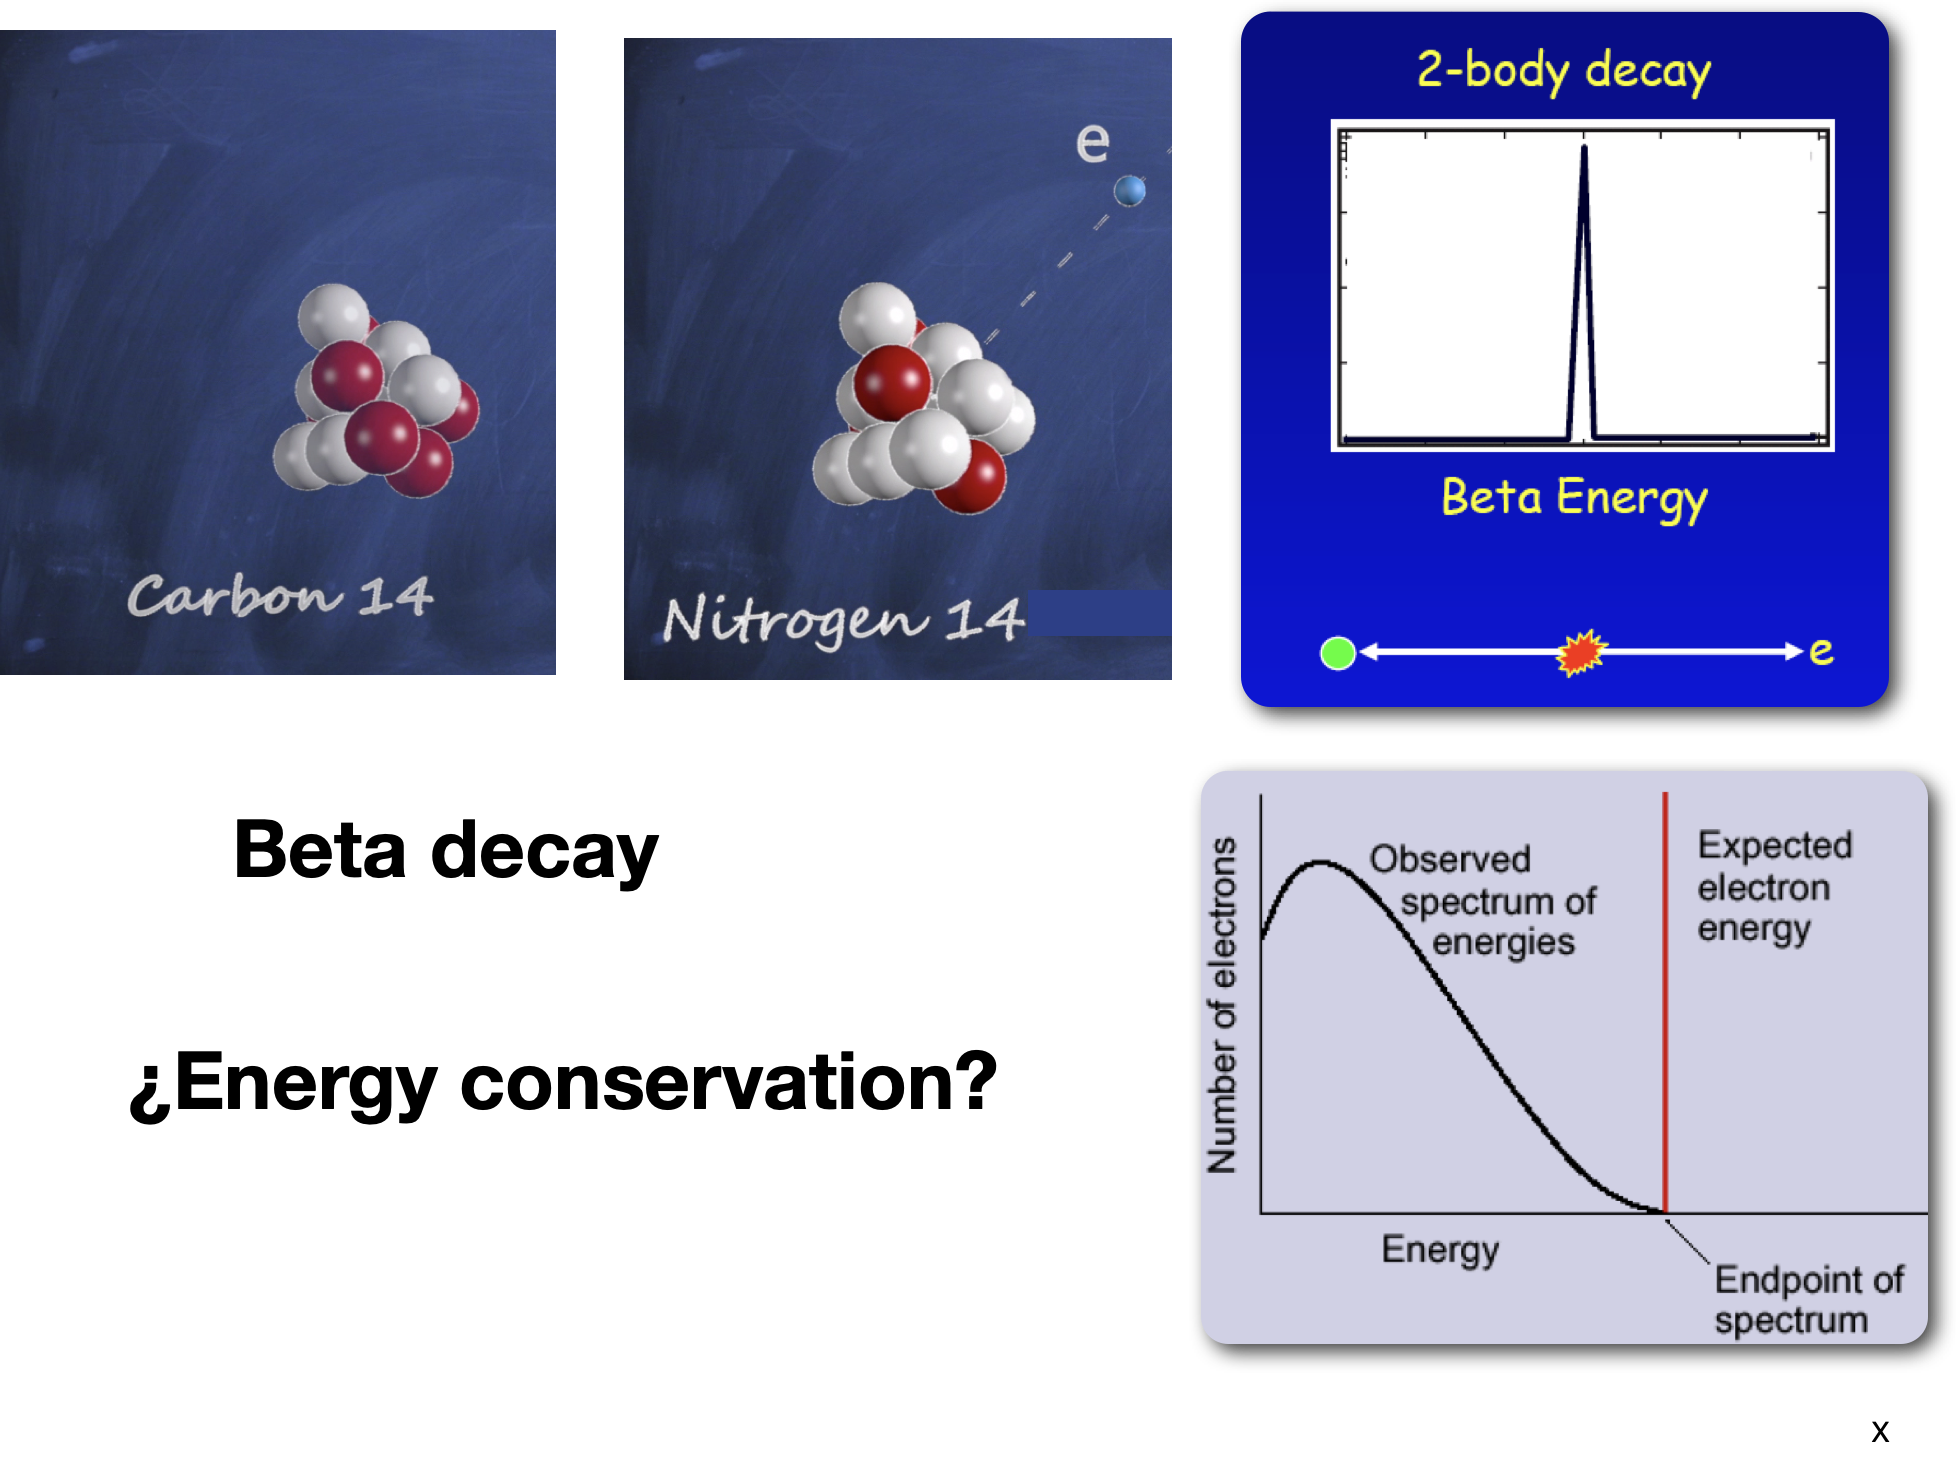
\includegraphics[scale=0.3]{img/betaDecay.png}
\end{frame}

\begin{frame}
\frametitle{Liebe Radioaktive Damen und Herren}
\begin{columns}
 
\column{0.5\textwidth}
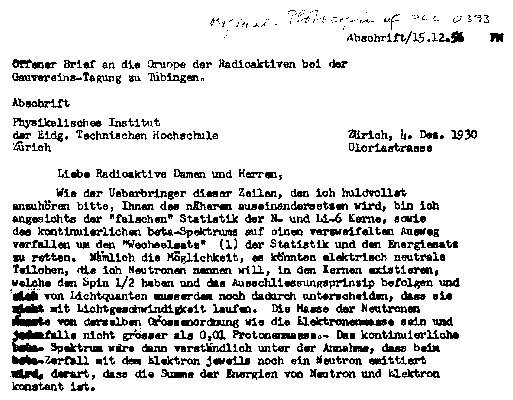
\includegraphics[scale=0.4]{img/liebe.png}
 
\column{0.2\textwidth}
\begin{block}{}
Dear Radioactive Ladies and Getlemen.

...because the continuous beta spectrum...I have hit upon a desperate remedy to save the law of conservation of energy.

\end{block}
\end{columns}
\end{frame}


\begin{frame}
\frametitle{I do not believe in neutrinos}
\begin{columns}
\column{0.35\textwidth}
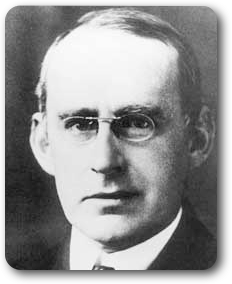
\includegraphics[scale=0.3]{img/eddington.png}
 
 \column{0.6\textwidth}
%\begin{block}{}
Sir Arthur Eddington: ``Just now nuclear physicists are writing a great deal about hypothetical particles called neutrinos supposed to account for certain peculiar facts observed in $\beta$-ray disintegration. We can perhaps best describe the neutrinos as little bits of spin-energy that have got detached. I am not much impressed by the neutrino theory. \alert{In an ordinary way I might say that I do not believe in neutrinos}... But I have to reflect that a physicist may be an artist, and you never know where you are with artists. My old-fashioned kind of disbelief in neutrinos is scarcely enough. \alert{Dare I say that experimental physicists will not have sufficient ingenuity to make neutrinos?"}

%\end{block}
\end{columns}
\end{frame}

\begin{frame}
\frametitle{The discovery of neutrinos}

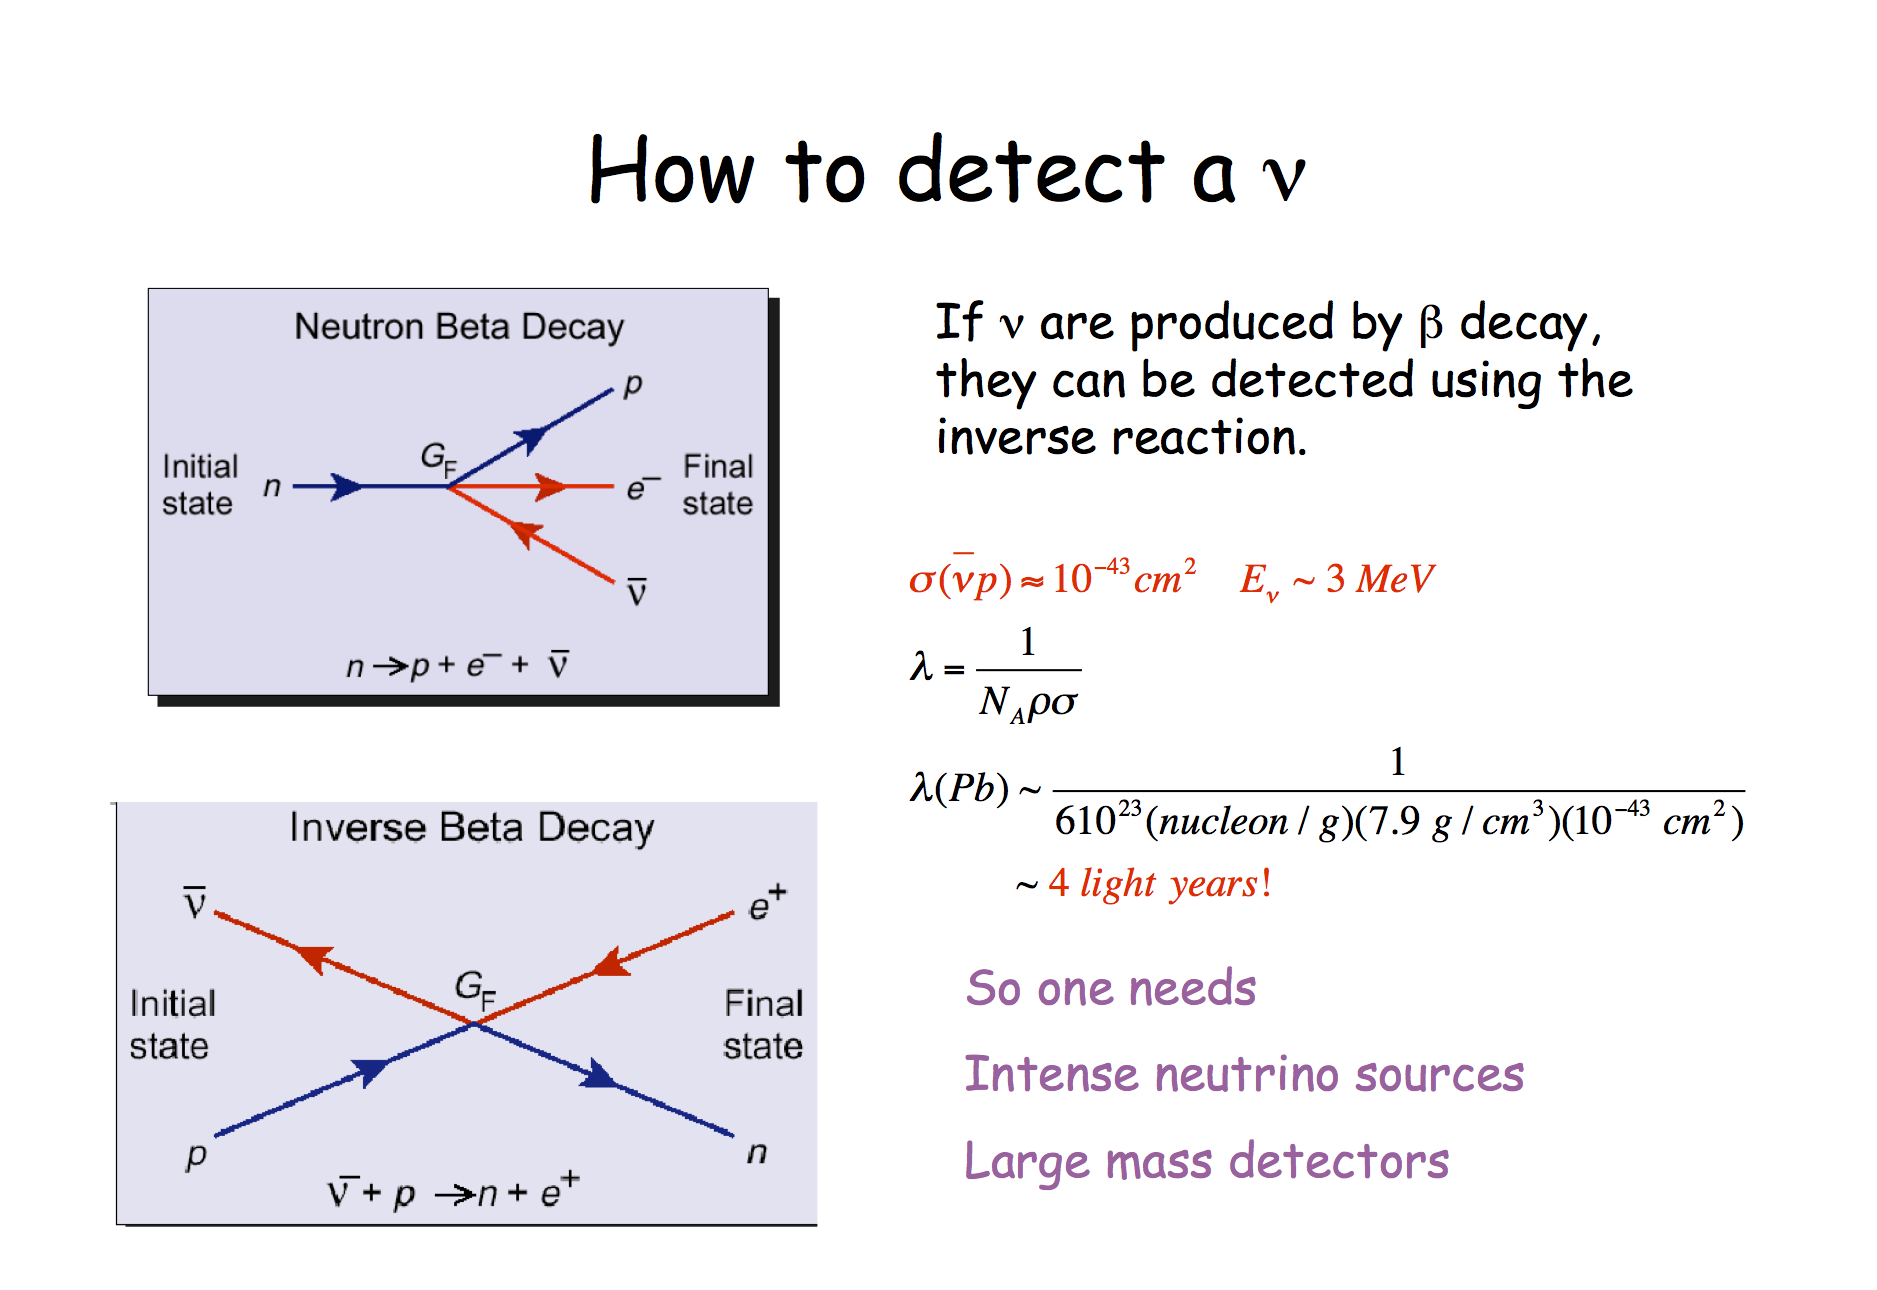
\includegraphics[scale=0.3]{img/DetectNeutrinos.png}

\end{frame}

\begin{frame}

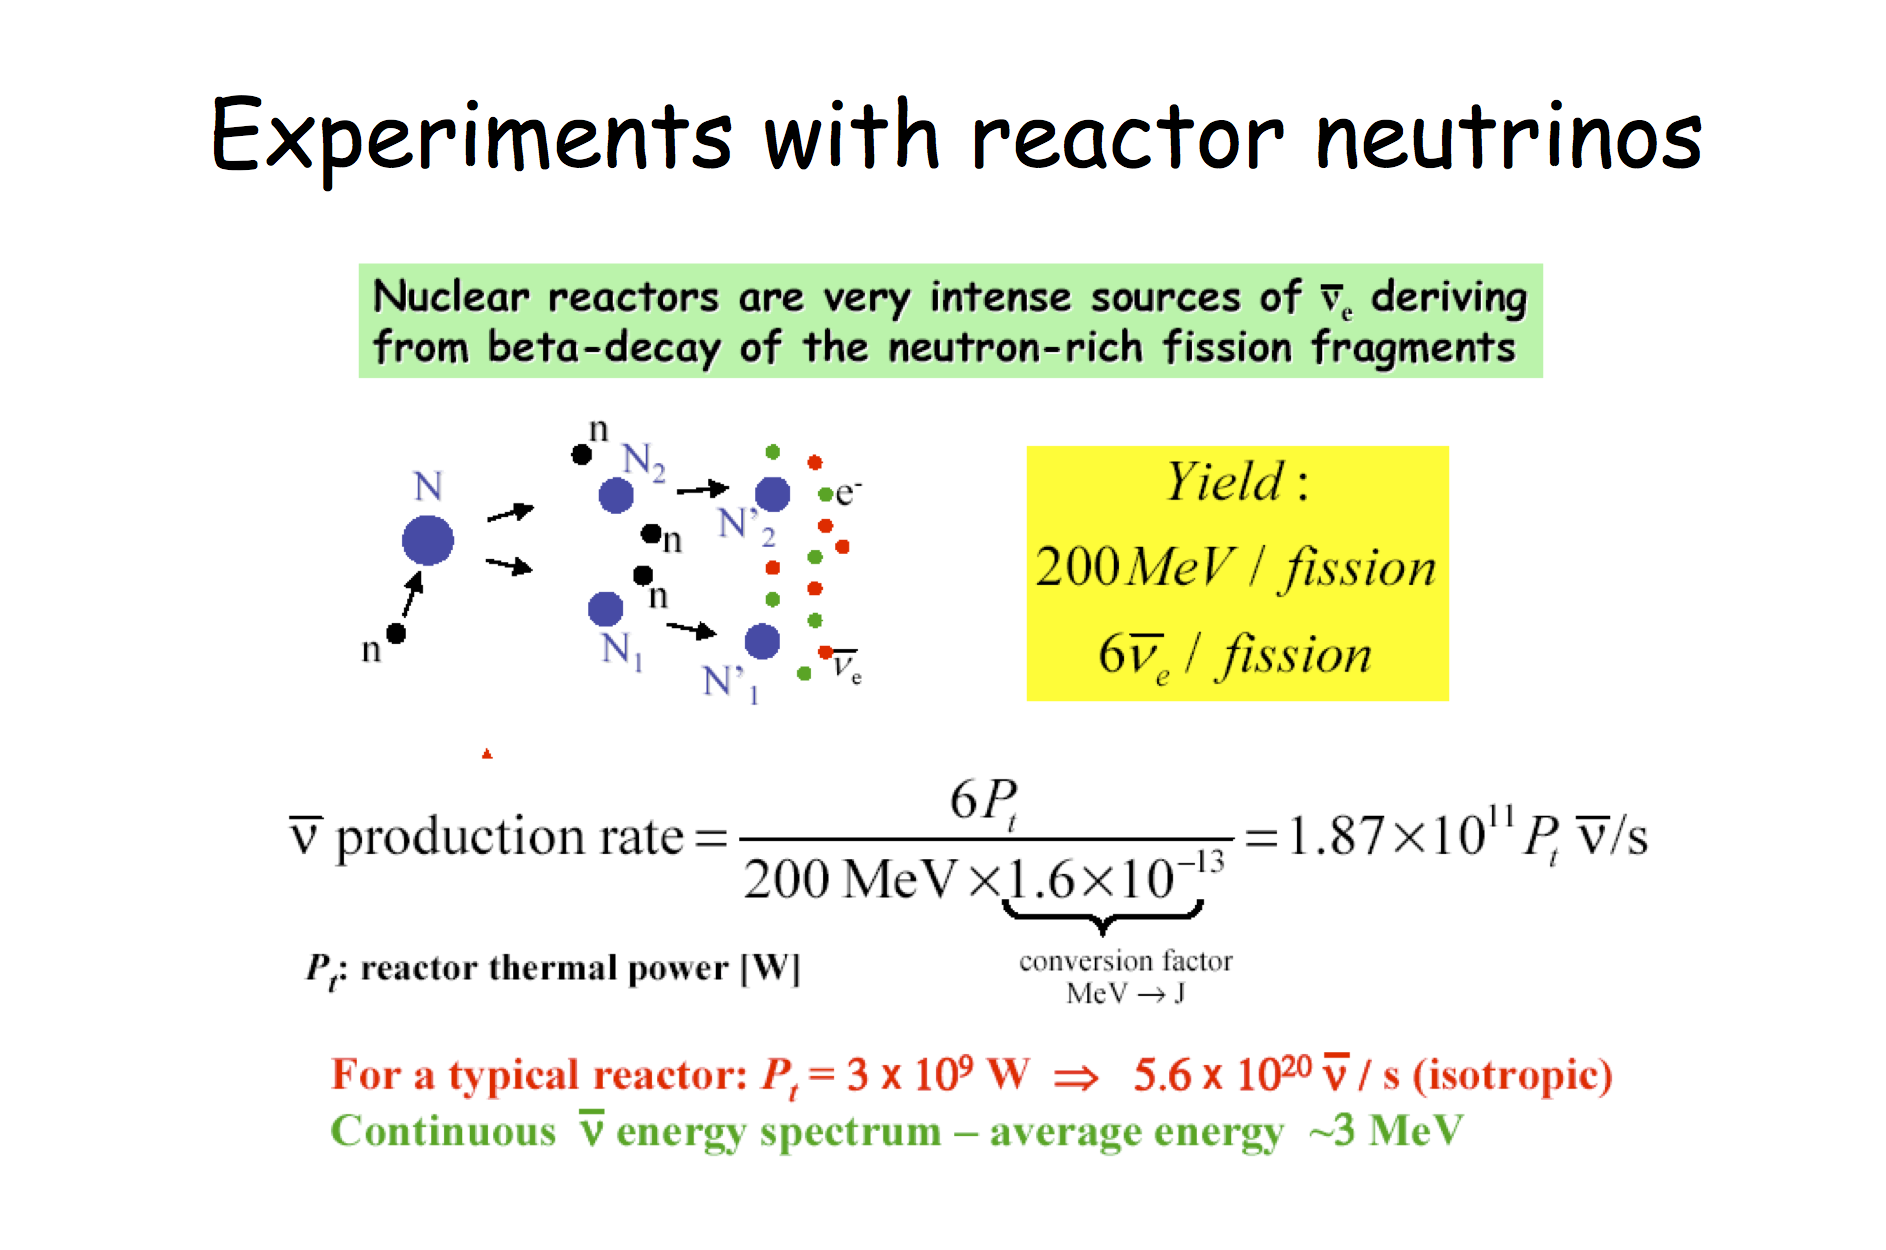
\includegraphics[scale=0.35]{img/ReactorNeutrinos.png}

\end{frame}

\begin{frame}
\frametitle{Reines, Cowen and delayed neutrons}
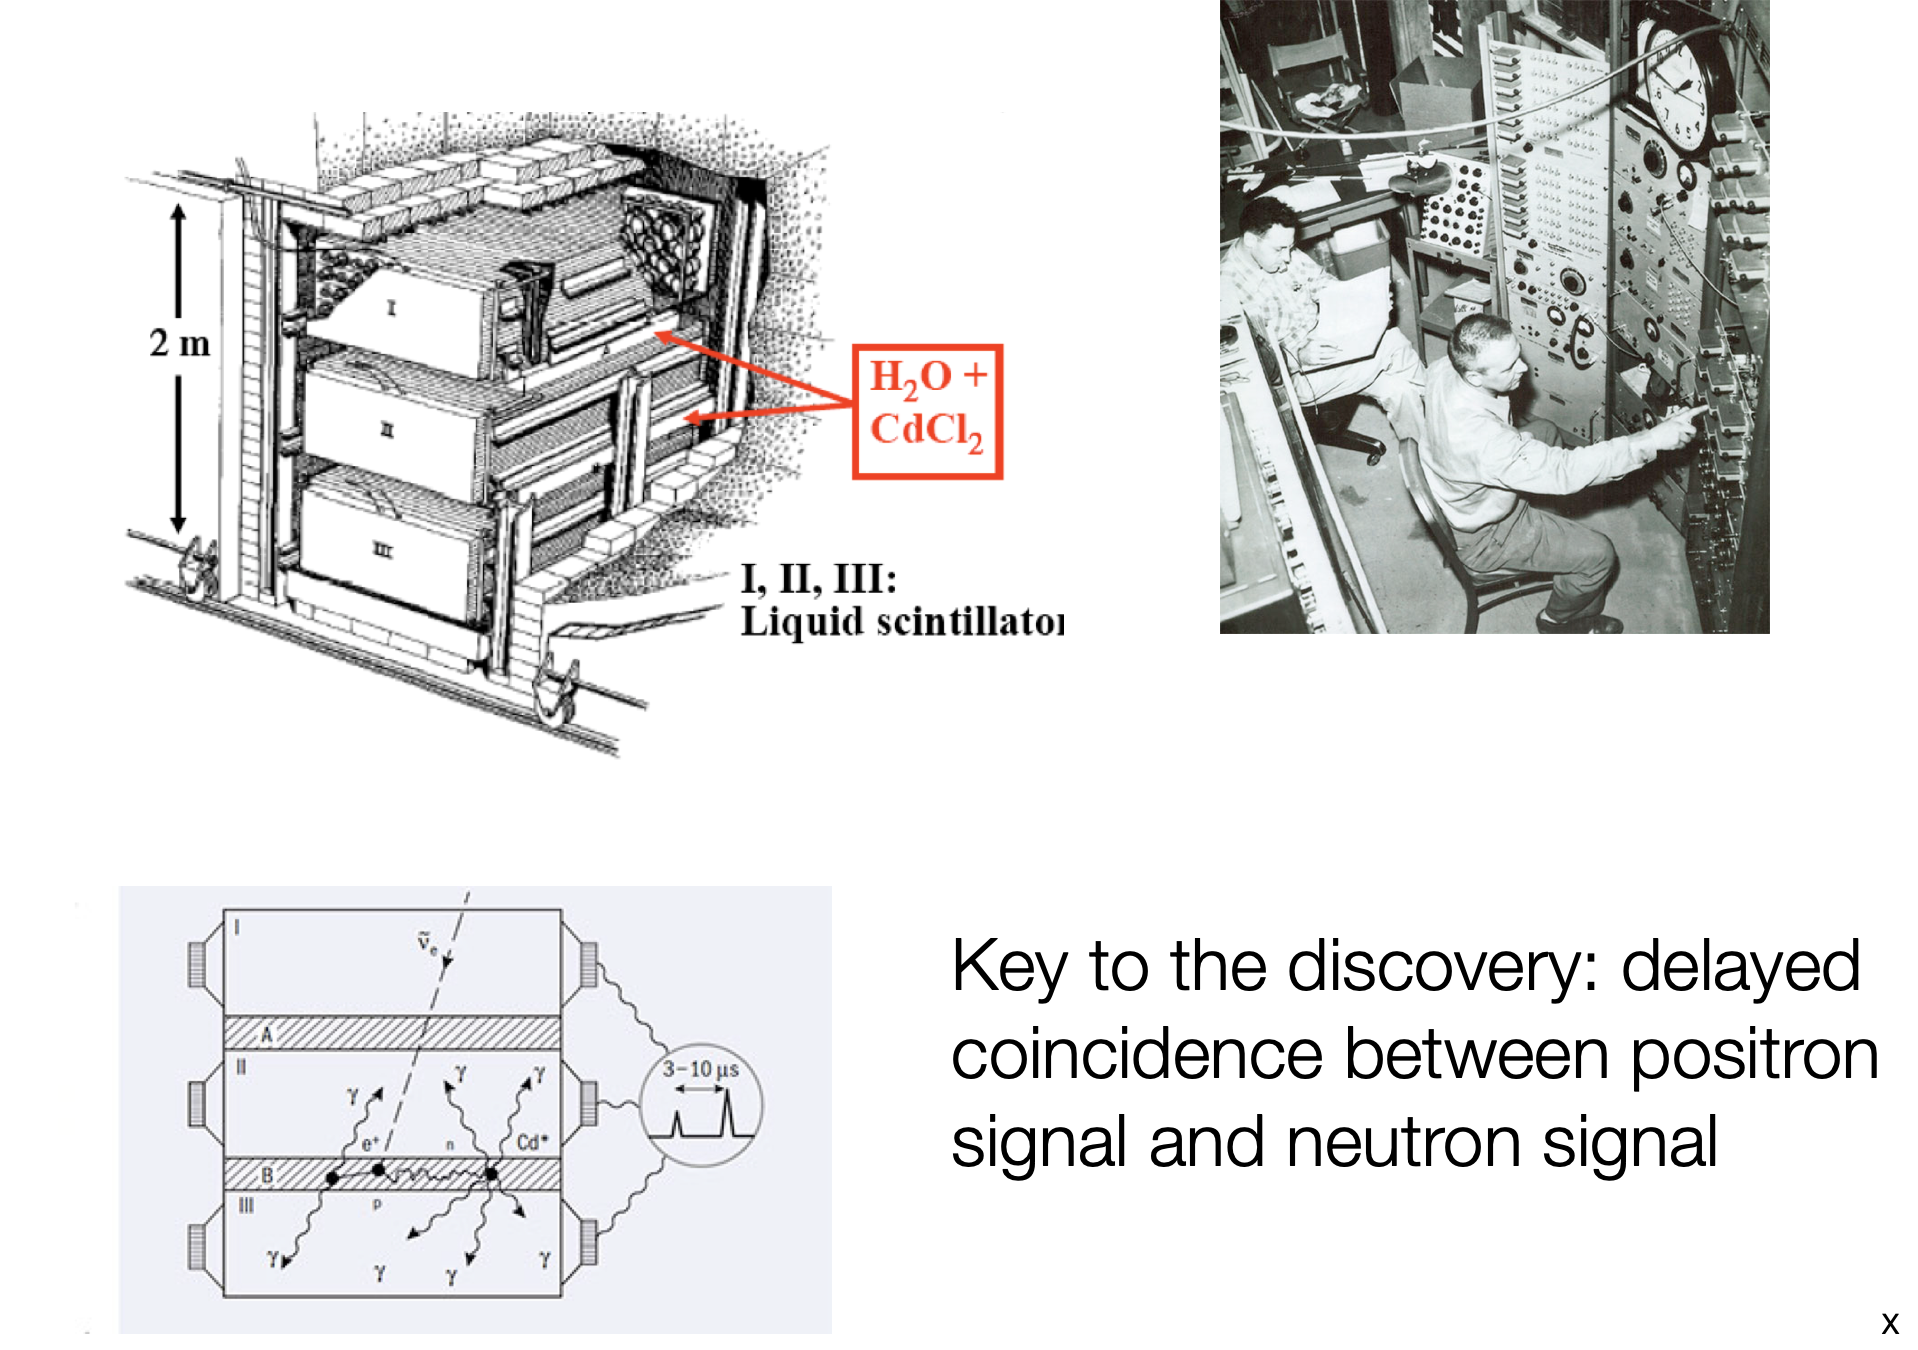
\includegraphics[scale=0.35]{img/ReinesCowen.png}

\end{frame}

%\begin{frame}
%
%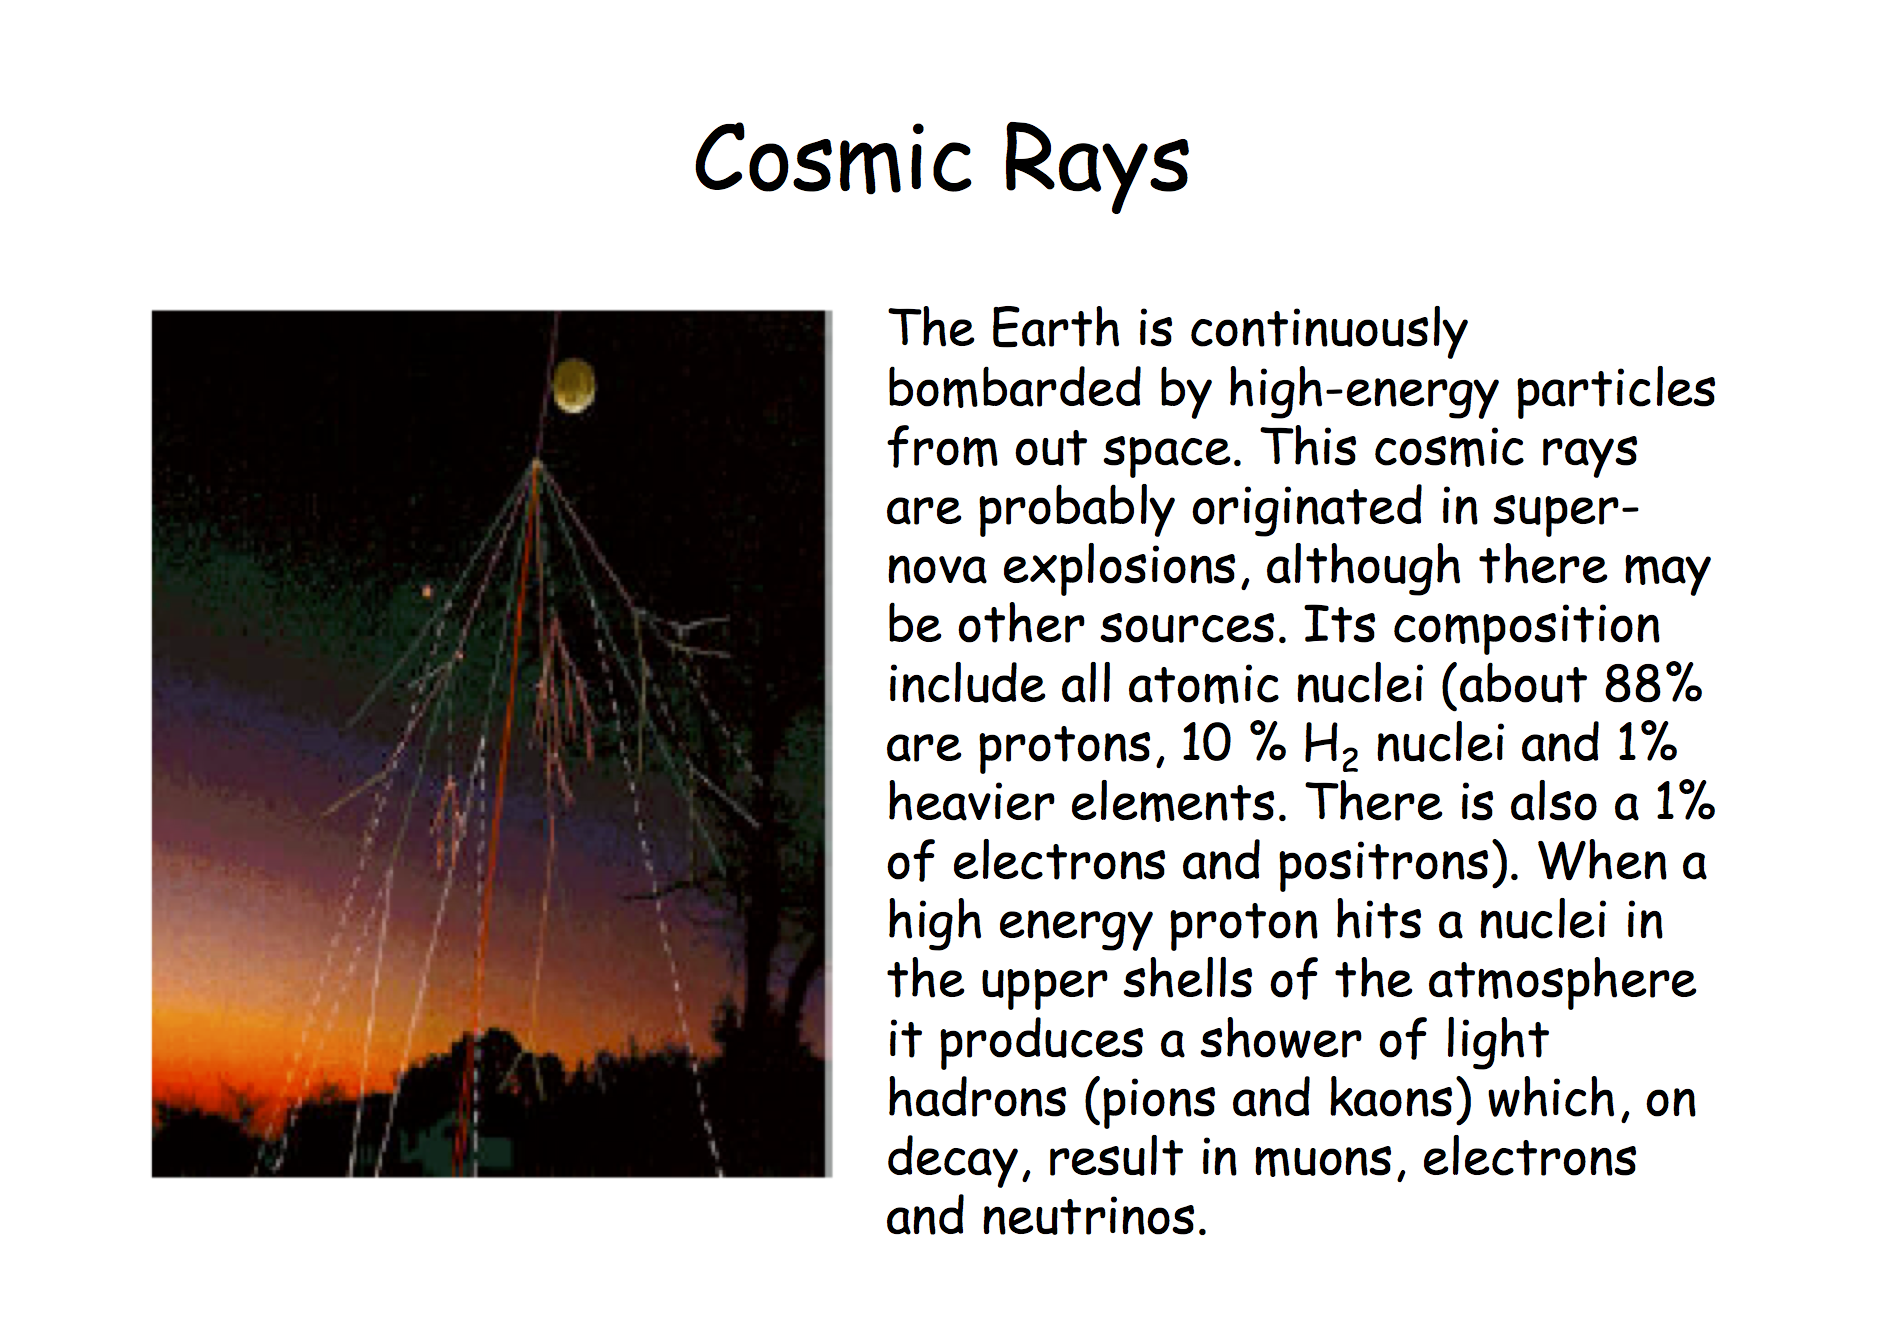
\includegraphics[scale=0.35]{CosmicRays.png}
%
%\end{frame}
%\begin{frame}
%
%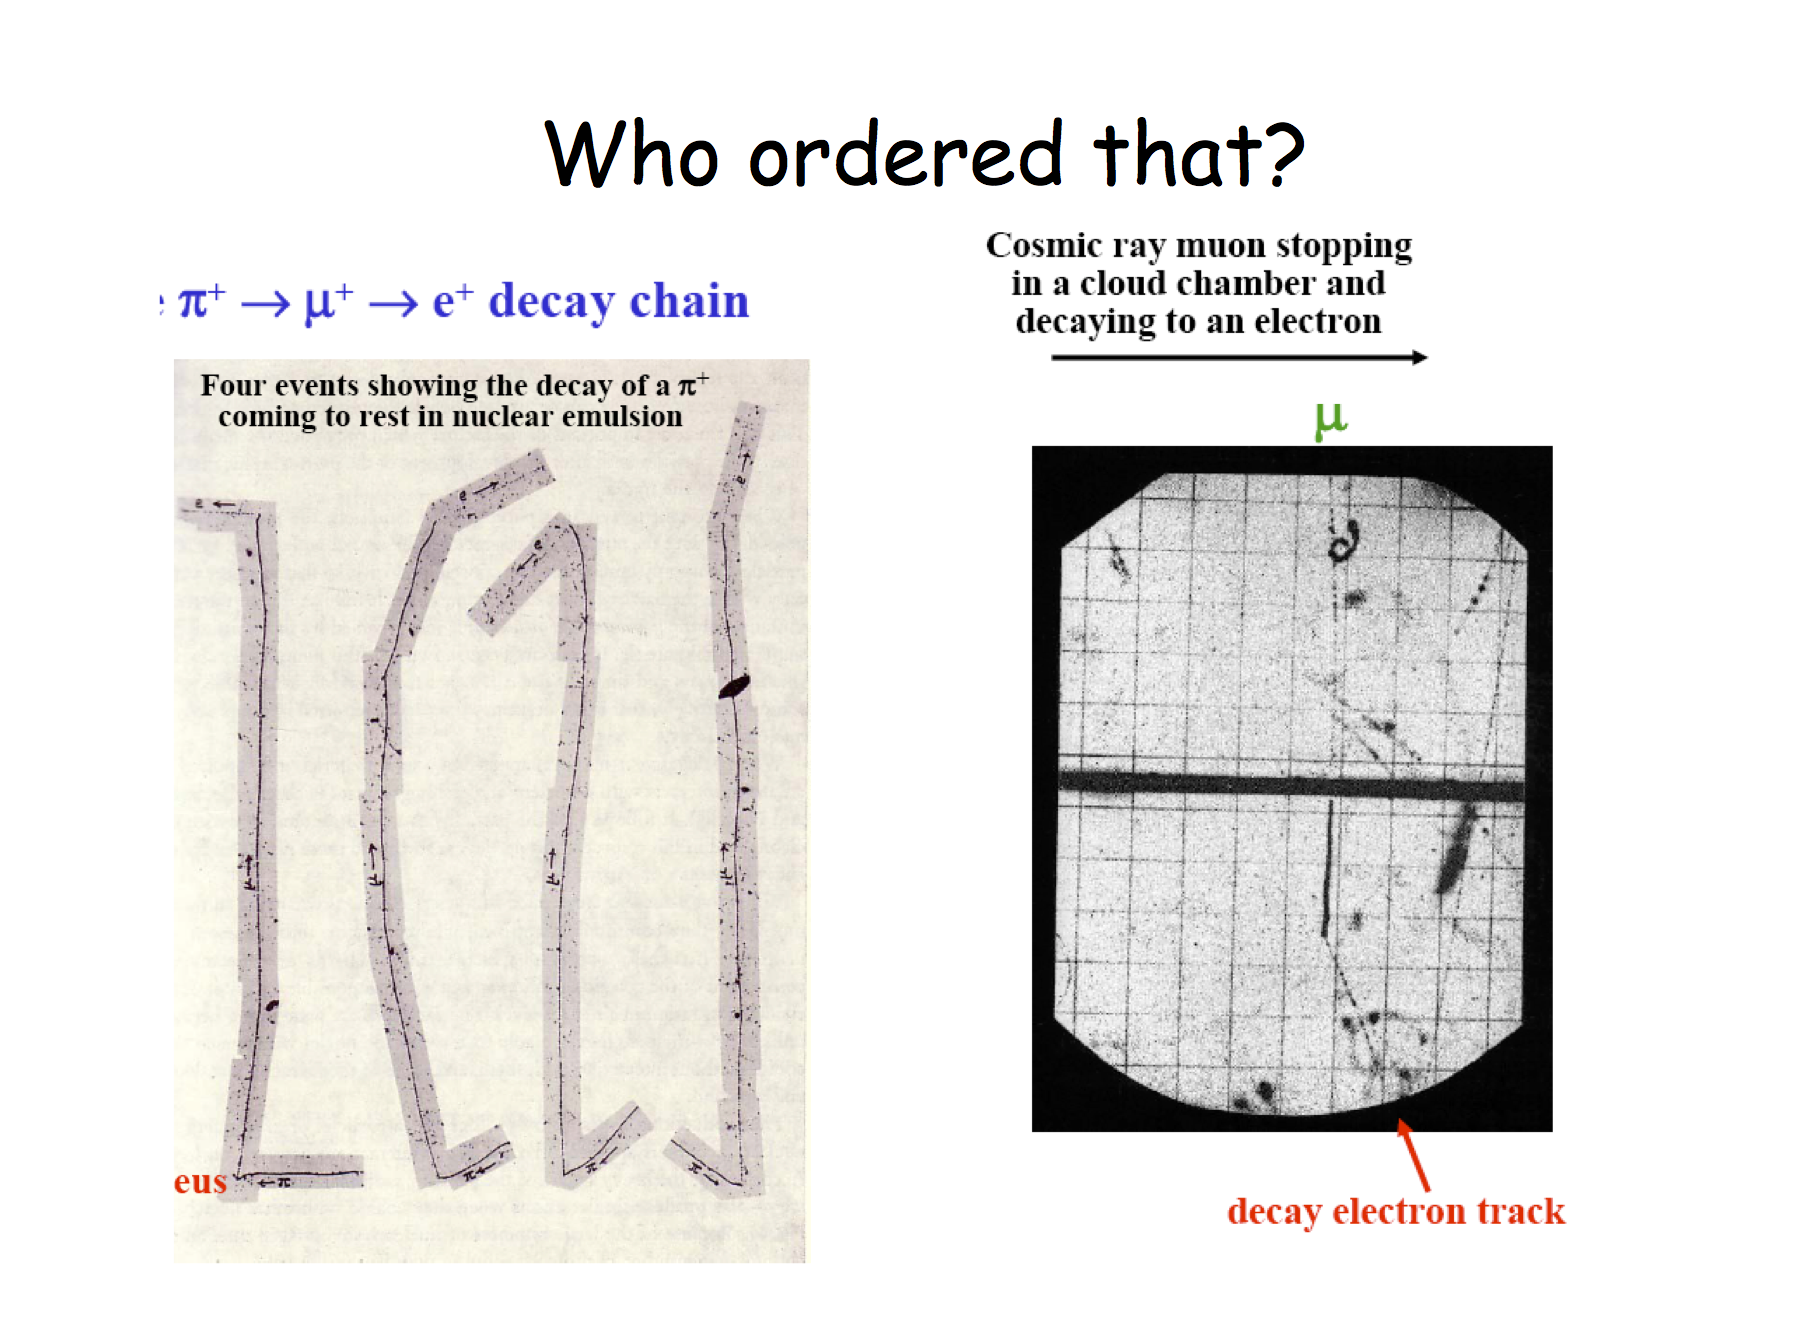
\includegraphics[scale=0.35]{WhoOrderedThat.png}
%
%\end{frame}
%\begin{frame}
%
%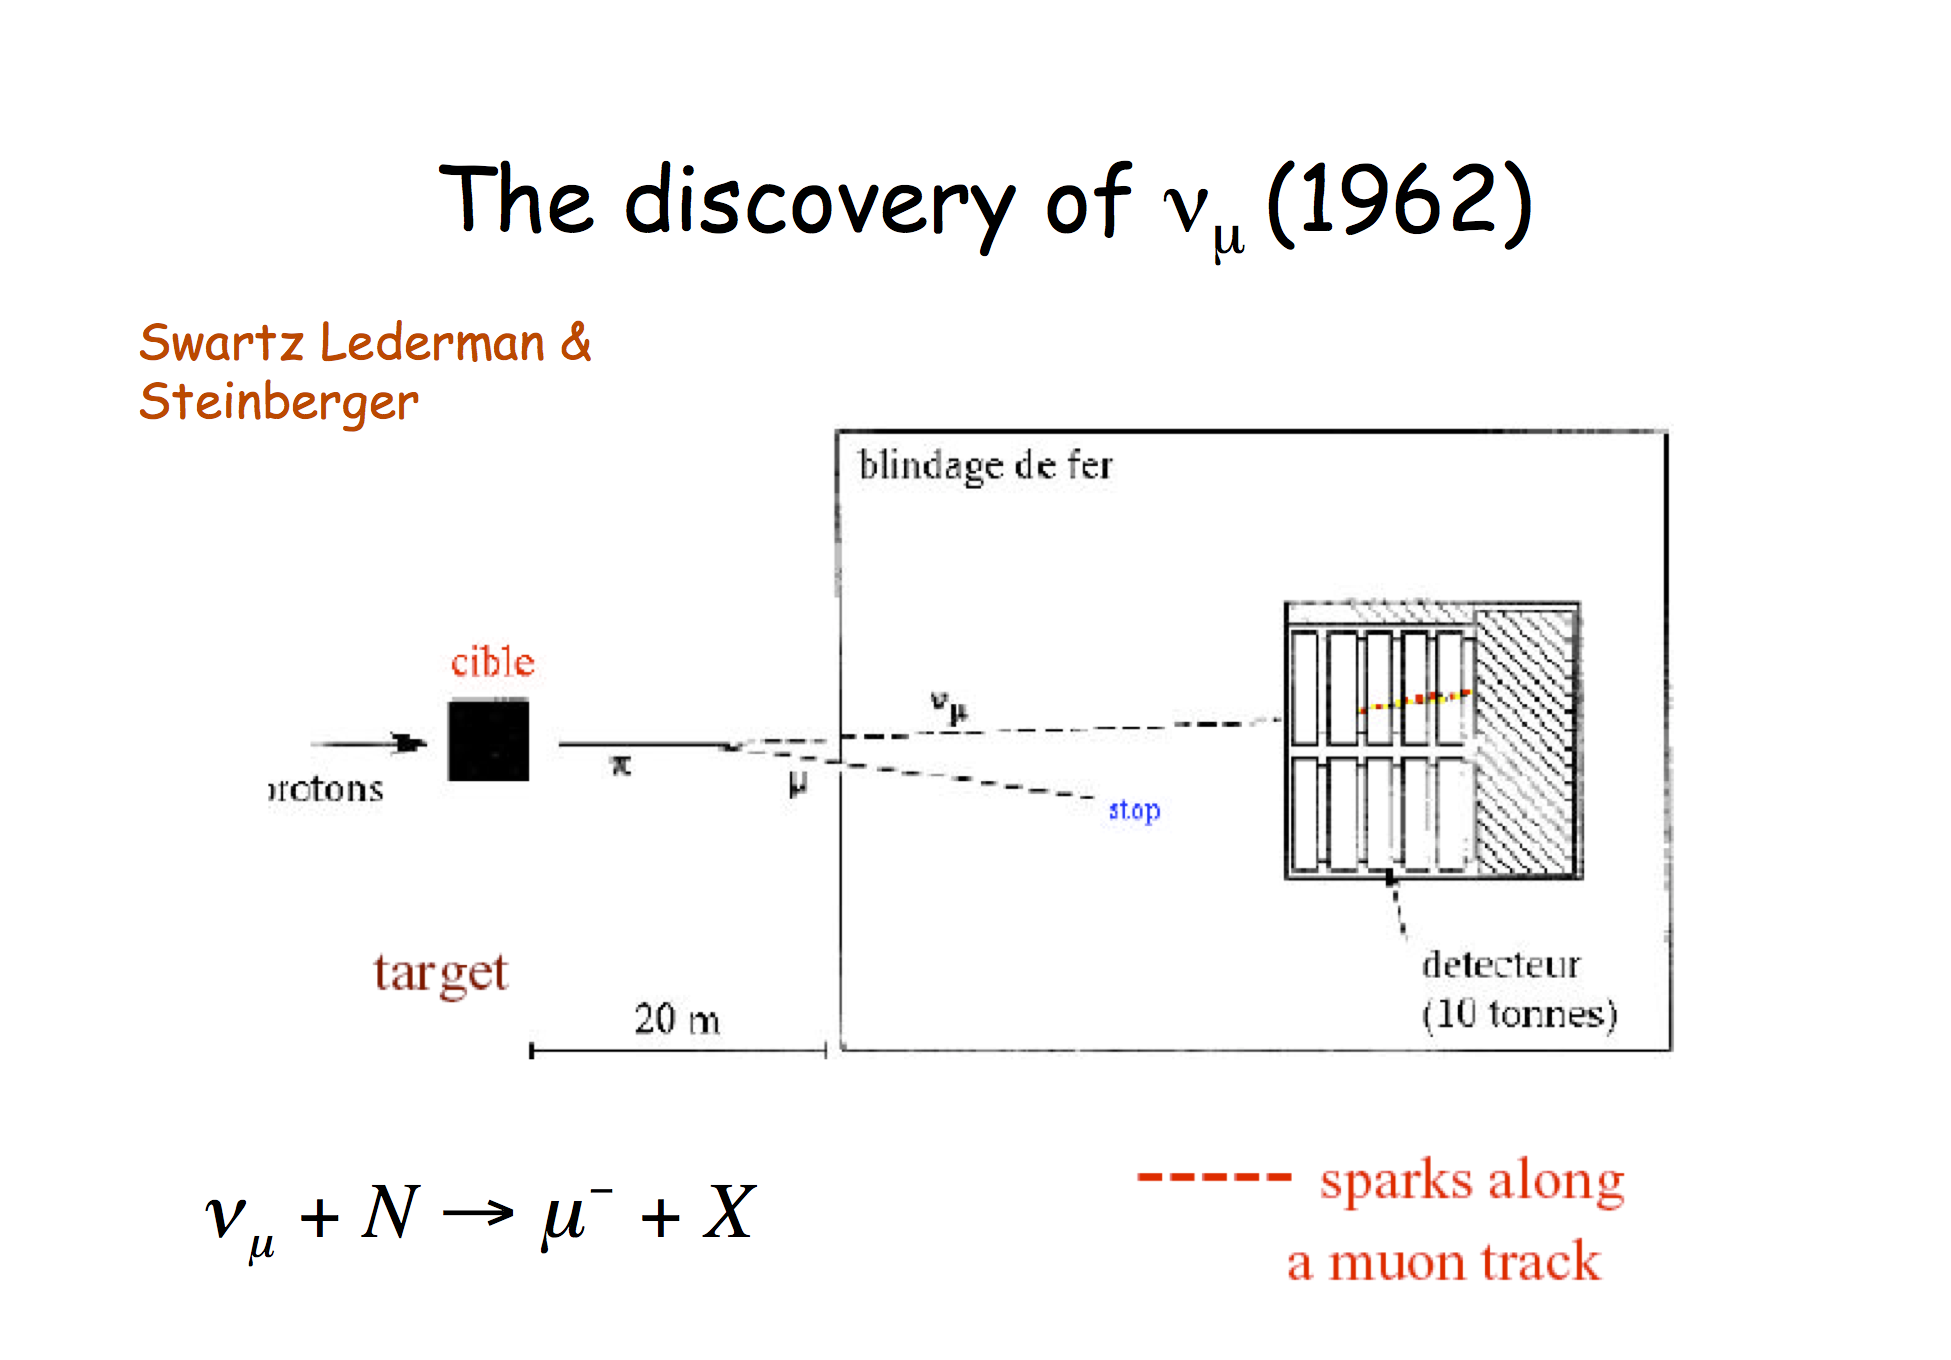
\includegraphics[scale=0.35]{DiscoveryNumu.png}
%
%\end{frame}
%\begin{frame}
%
%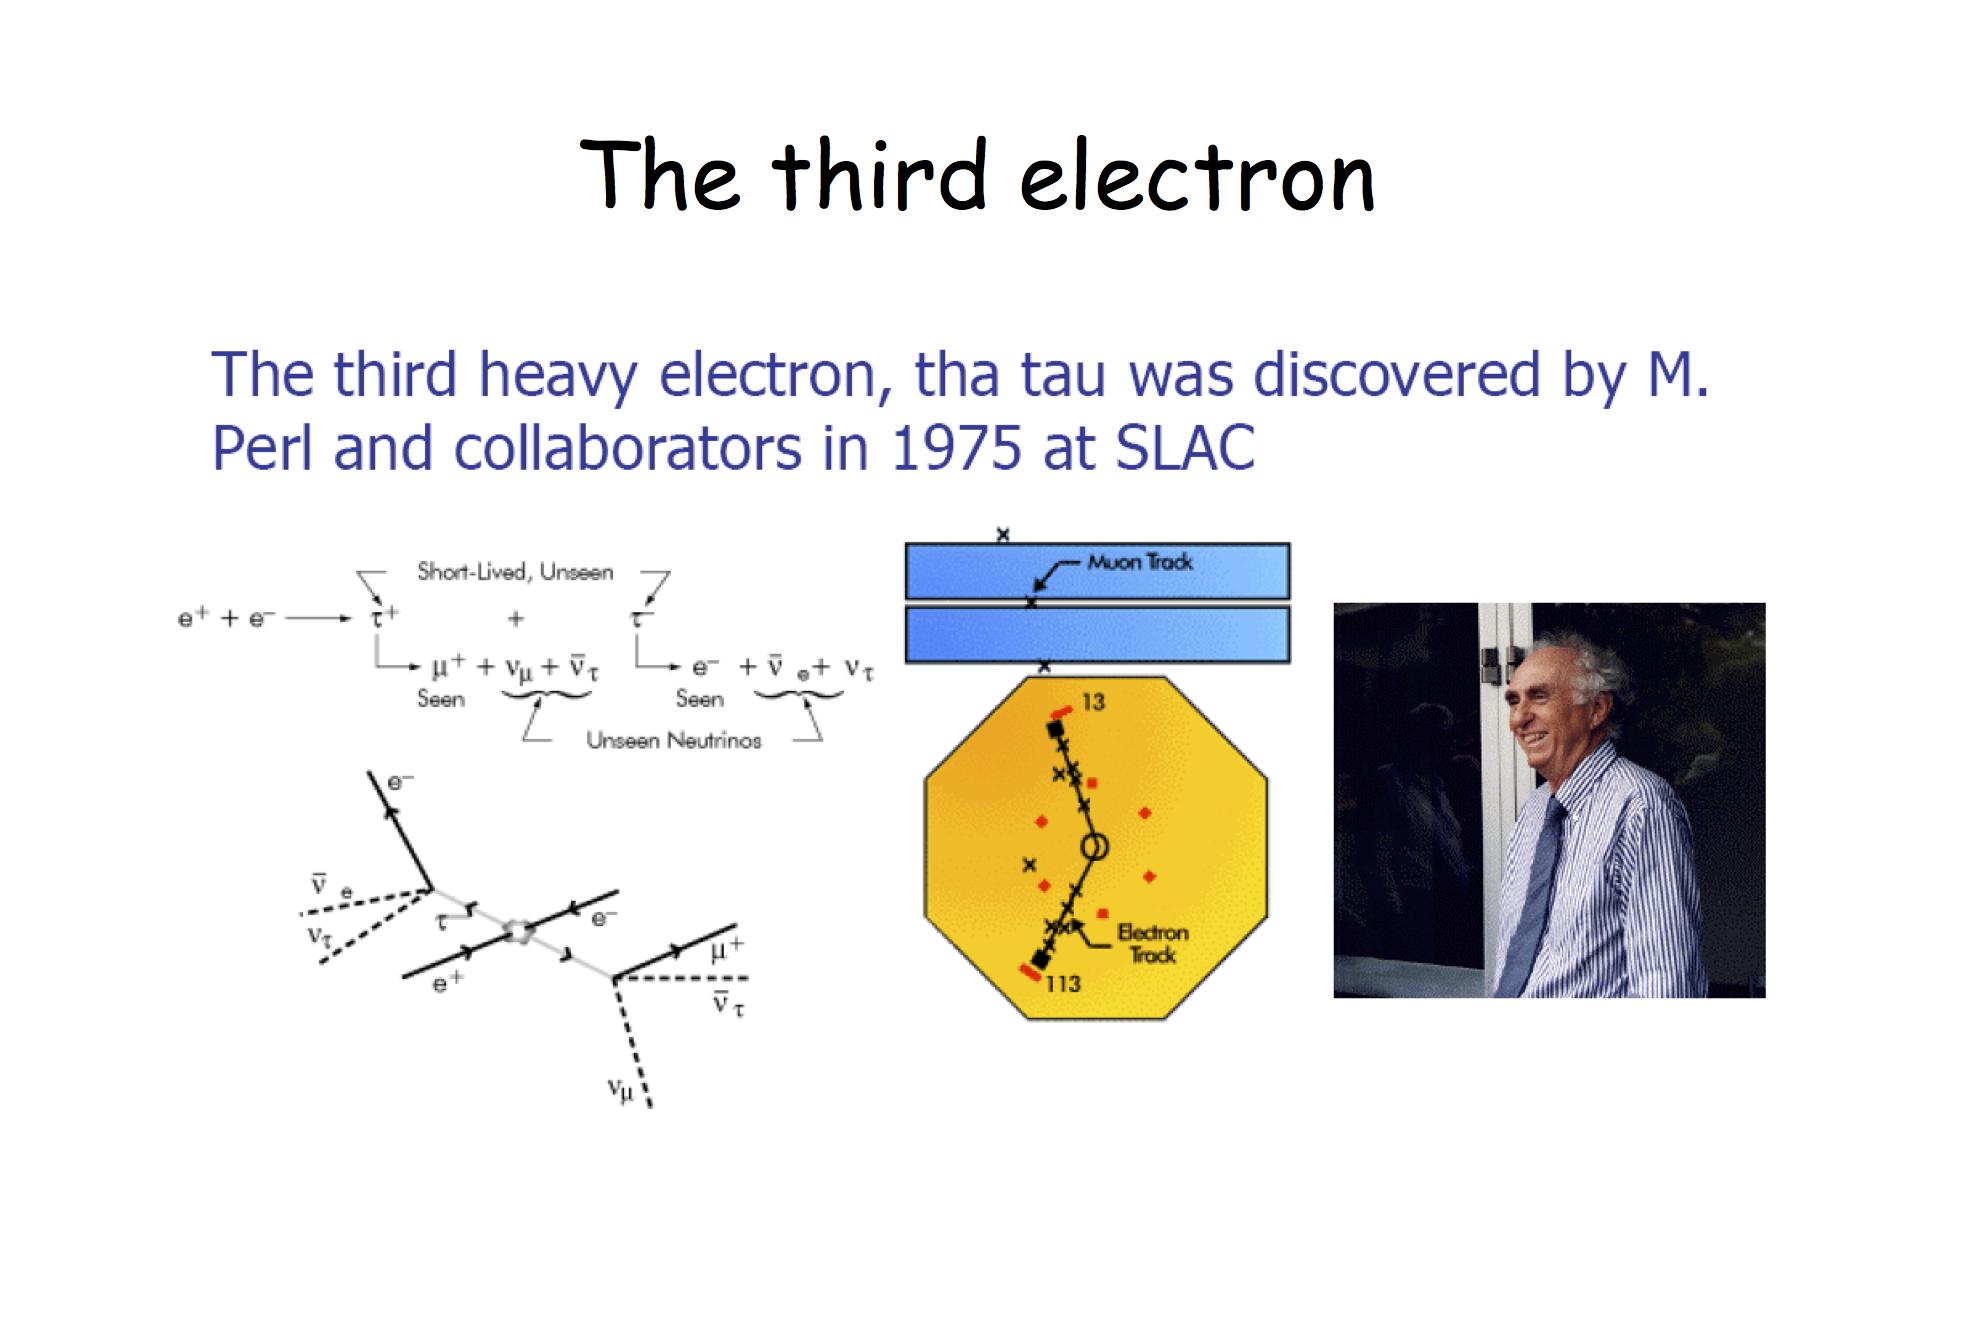
\includegraphics[scale=0.35]{tau.png}
%
%\end{frame}
%\begin{frame}
%
%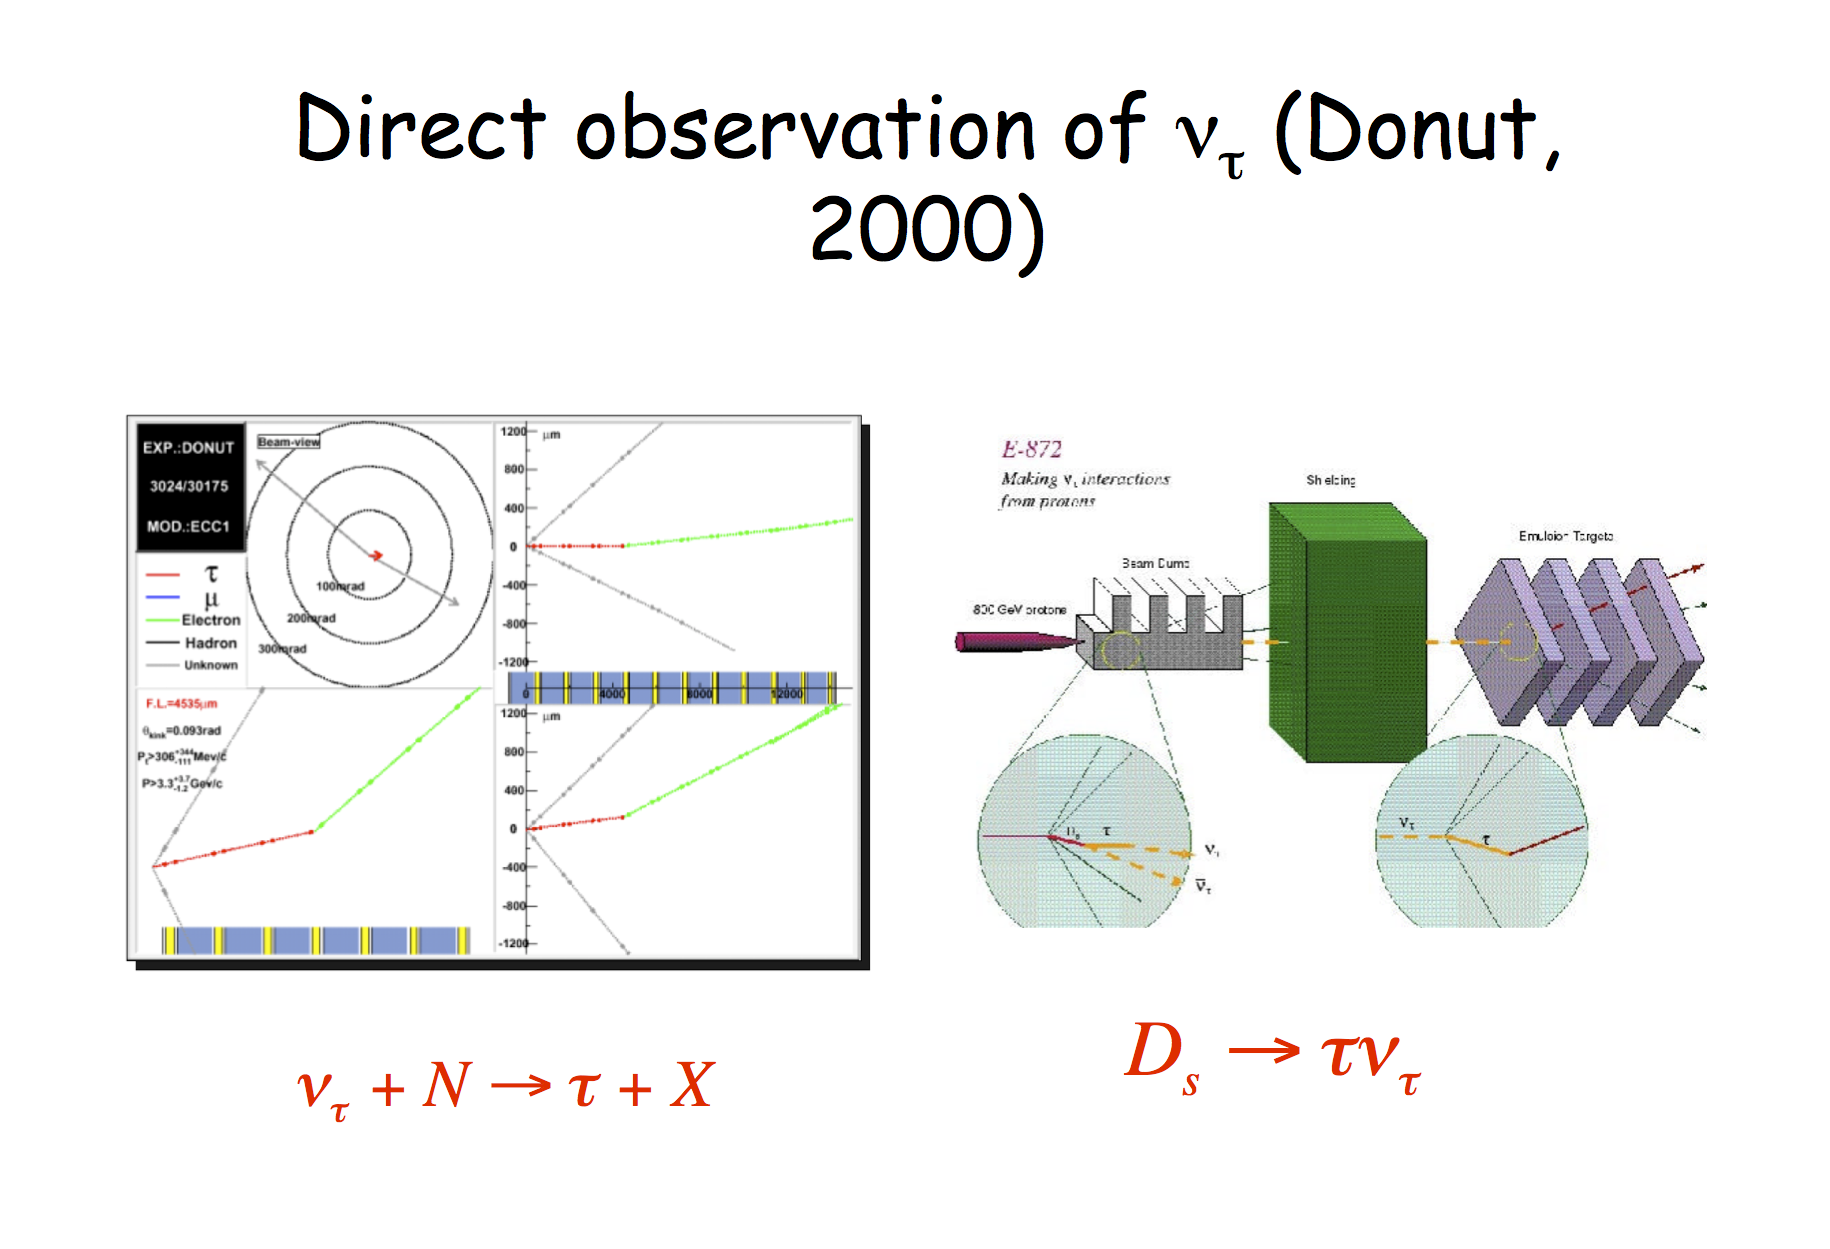
\includegraphics[scale=0.35]{DirectNuTau.png}
%
%\end{frame}
\begin{frame}
\frametitle{Neutrinos everywhere}
\begin{columns}
\column{0.35\textwidth}
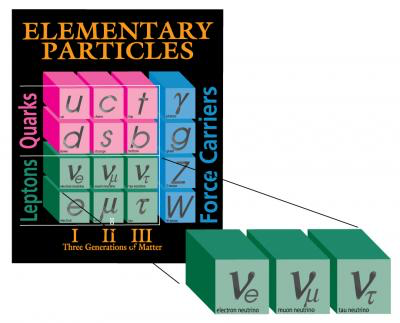
\includegraphics[scale=0.25]{img/Generations2.png}

Two heavy electrons (the $\mu$~and the $\tau$) have been discovered, each one accompanied with its own neutrino. For reasons yet unknown to us, Nature has chosen to produce three copies of the elementary fermions, identical except for their mass. 
 
 \column{0.6\textwidth}
%\begin{block}{}
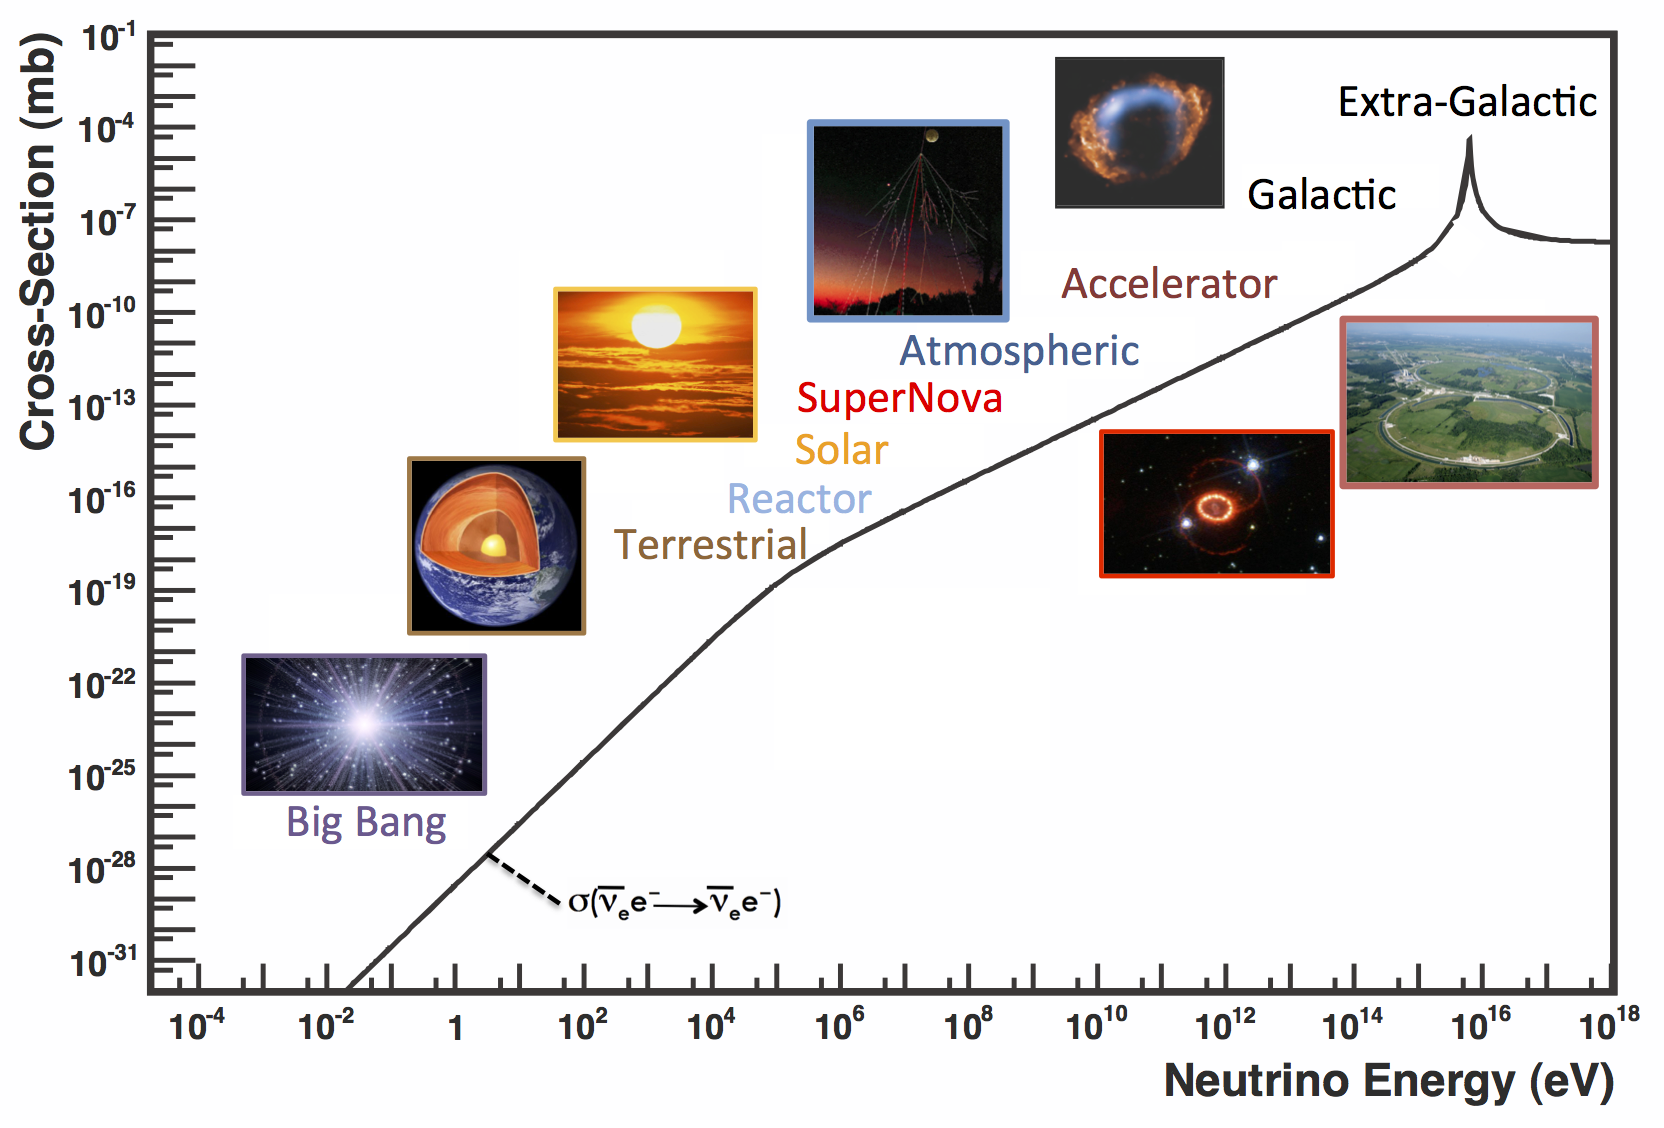
\includegraphics[scale=0.25]{img/NeutrinoSources.png}

Neutrinos are everywhere and we have produced and detected them by the millions. Eddington would not have made a living as a prophet (who does?)


%\end{block}
\end{columns}




\end{frame}



\section{Through the looking glass}
\begin{frame}
\frametitle{Neutrinos through the looking glass}

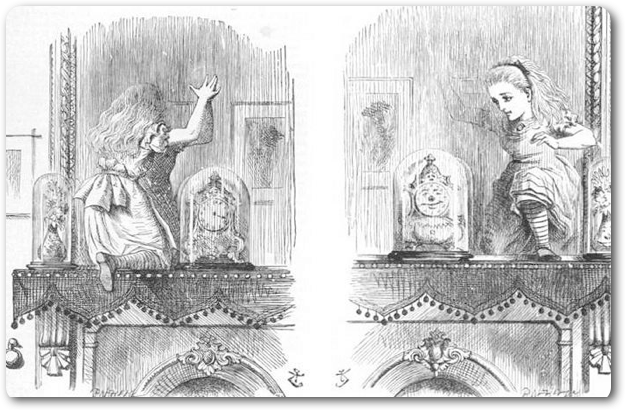
\includegraphics[scale=0.4]{img/Alice.png}

\end{frame}


\begin{frame}
\frametitle{Parity}
\begin{columns}
\column{0.5\textwidth}

\includegraphics[scale=0.45]{img/ParityCartoon.png}


The parity transformation changes a right-handed coordinate system into a left-handed one or vice versa. Two applications of the parity transformation restores the coordinate system to its original state.

It is a reasonable presupposition that nature should not care whether its coordinate system is right-handed or left-handed, \alert{but surprisingly, that turns out not to be so.}

\column{0.5\textwidth}
%\begin{block}{}
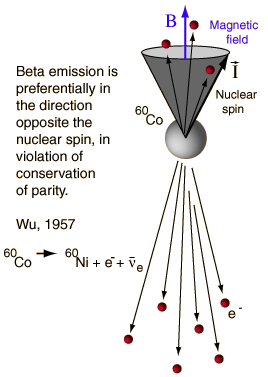
\includegraphics[scale=0.35]{img/wu.png}

In 1956, T. D. Lee and C. N. Yang predicted the non conservation of parity in the weak interaction. Their prediction was quickly tested when C. S. Wu and collaborators studied the beta decay of Cobalt-60 in 1957.

%\end{block}
\end{columns}

\end{frame}

%\begin{frame}
%\includegraphics[scale=0.35]{Cobalt.png}
%%wu.png
%\end{frame}
%GoldhaberExperiment.png
\begin{frame}
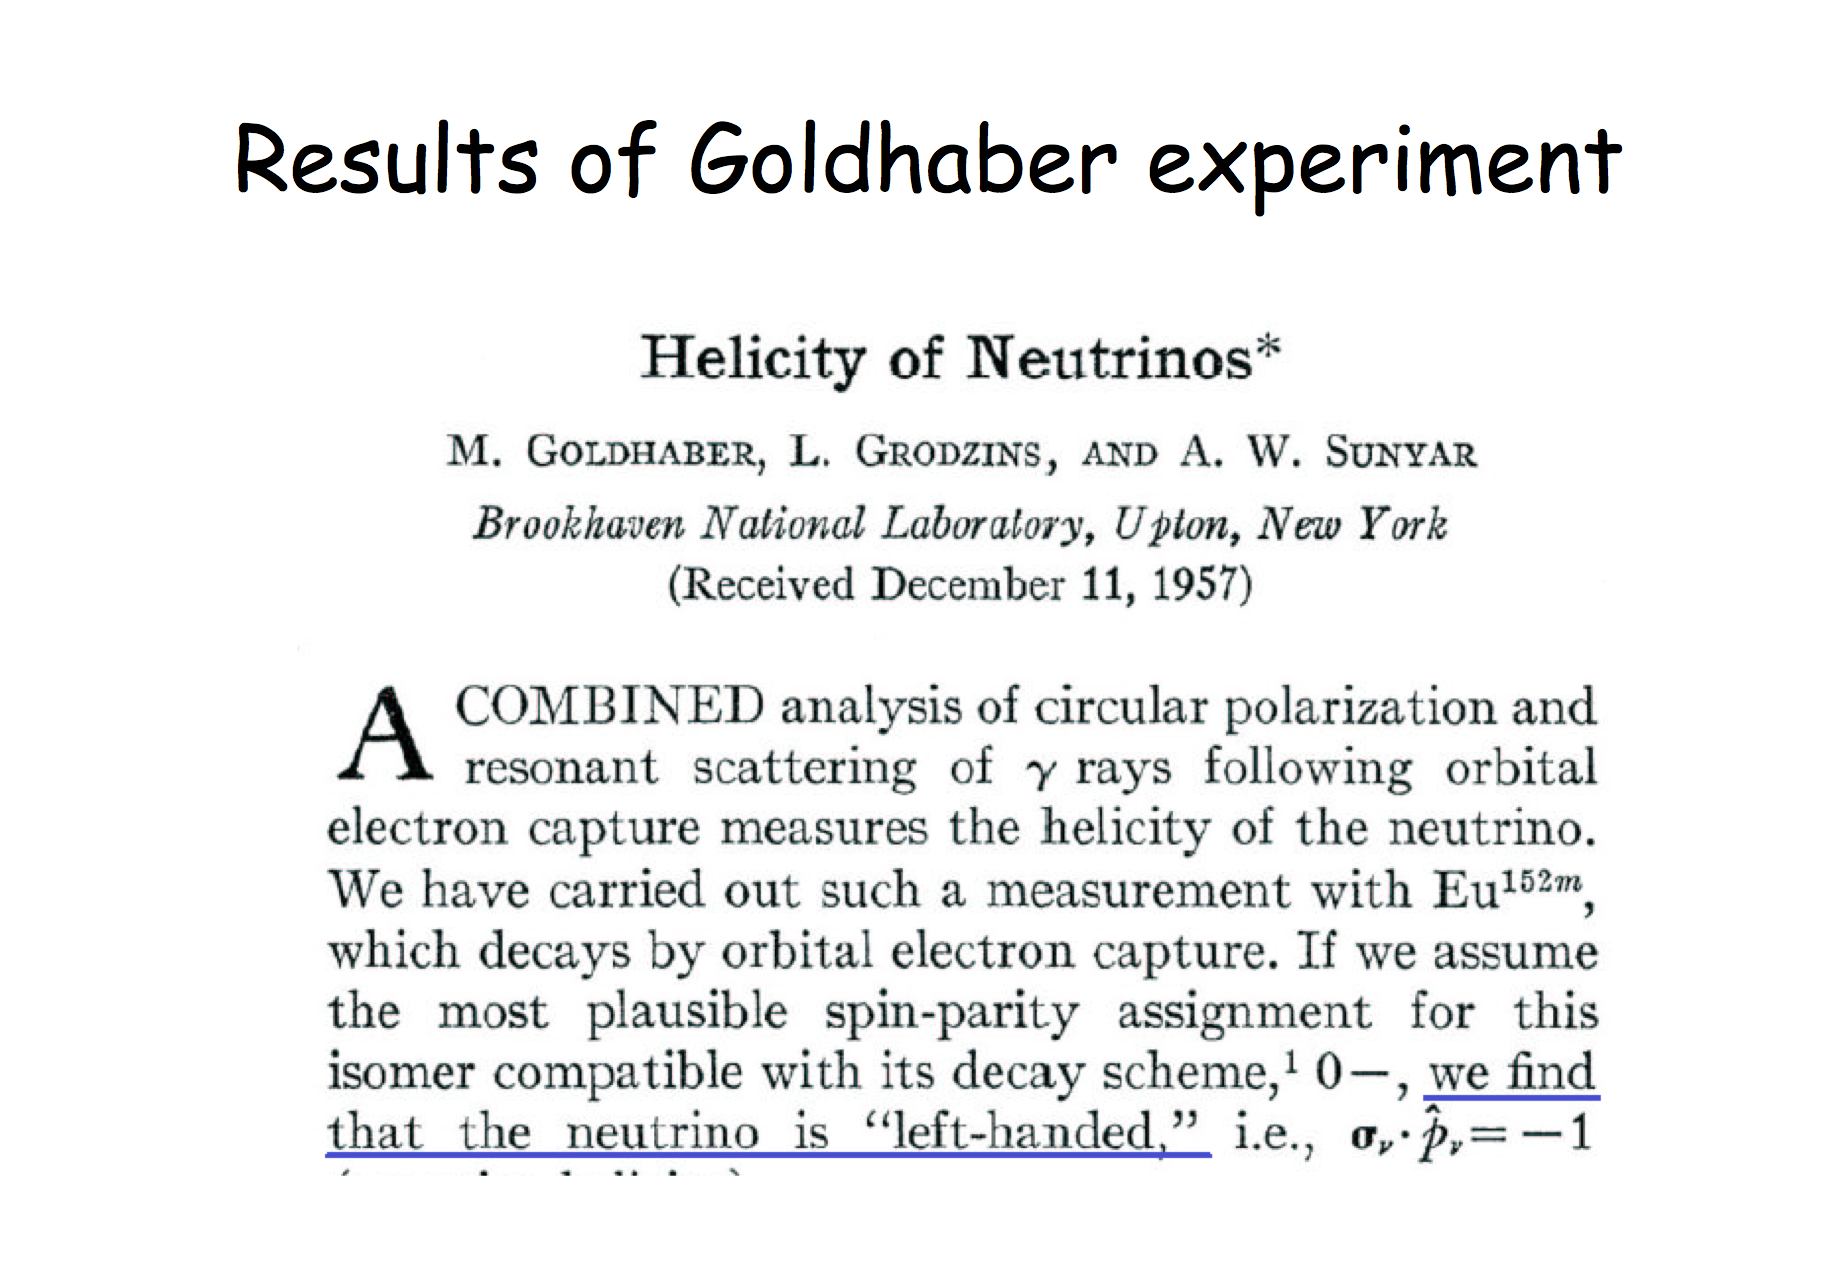
\includegraphics[scale=0.35]{img/Goldhaber.png}

\end{frame}

\begin{frame}
\frametitle{What do we talk about when we talk about helicity?}
\begin{columns}
\column{0.5\textwidth}
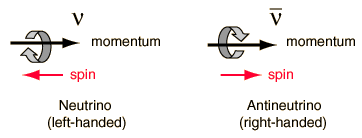
\includegraphics[scale=0.35]{img/NeutrinoHelicity.png}

Helicity is the spin projection in the direction of motion.
\[
h = \frac{\va{\sigma}\cdot \va{p}}{p}
\]
The Goldhaber experiment measured that neutrinos are left handed (spin opposed to motion, $h=-1$). The CPT theorem ensures that anti-neutrinos must be right-handed (spin along motion, $h=+1$).
\column{0.5\textwidth}

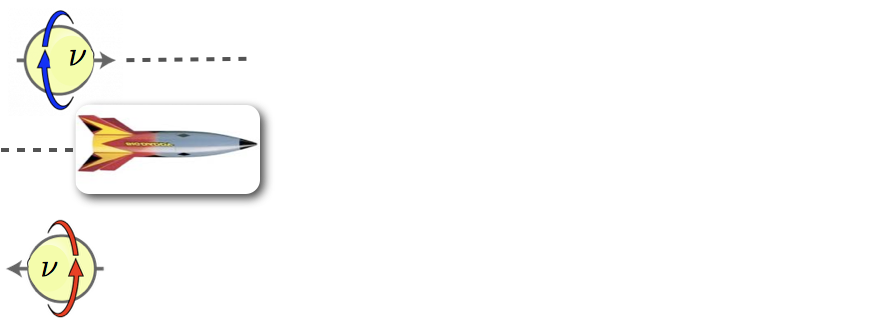
\includegraphics[scale=0.30]{img/neutrinoBoost2.png}

For massive particles, helicity depends on the reference frame and thus is not Lorentz invariant. One can always jump into a reference system faster than that of the particle and see its helicity flip.

But massless particles travel at the speed of light and cannot be overtaken. The helicity becomes a constant of motion. 
\end{columns}

\end{frame}

%
%\begin{frame}
%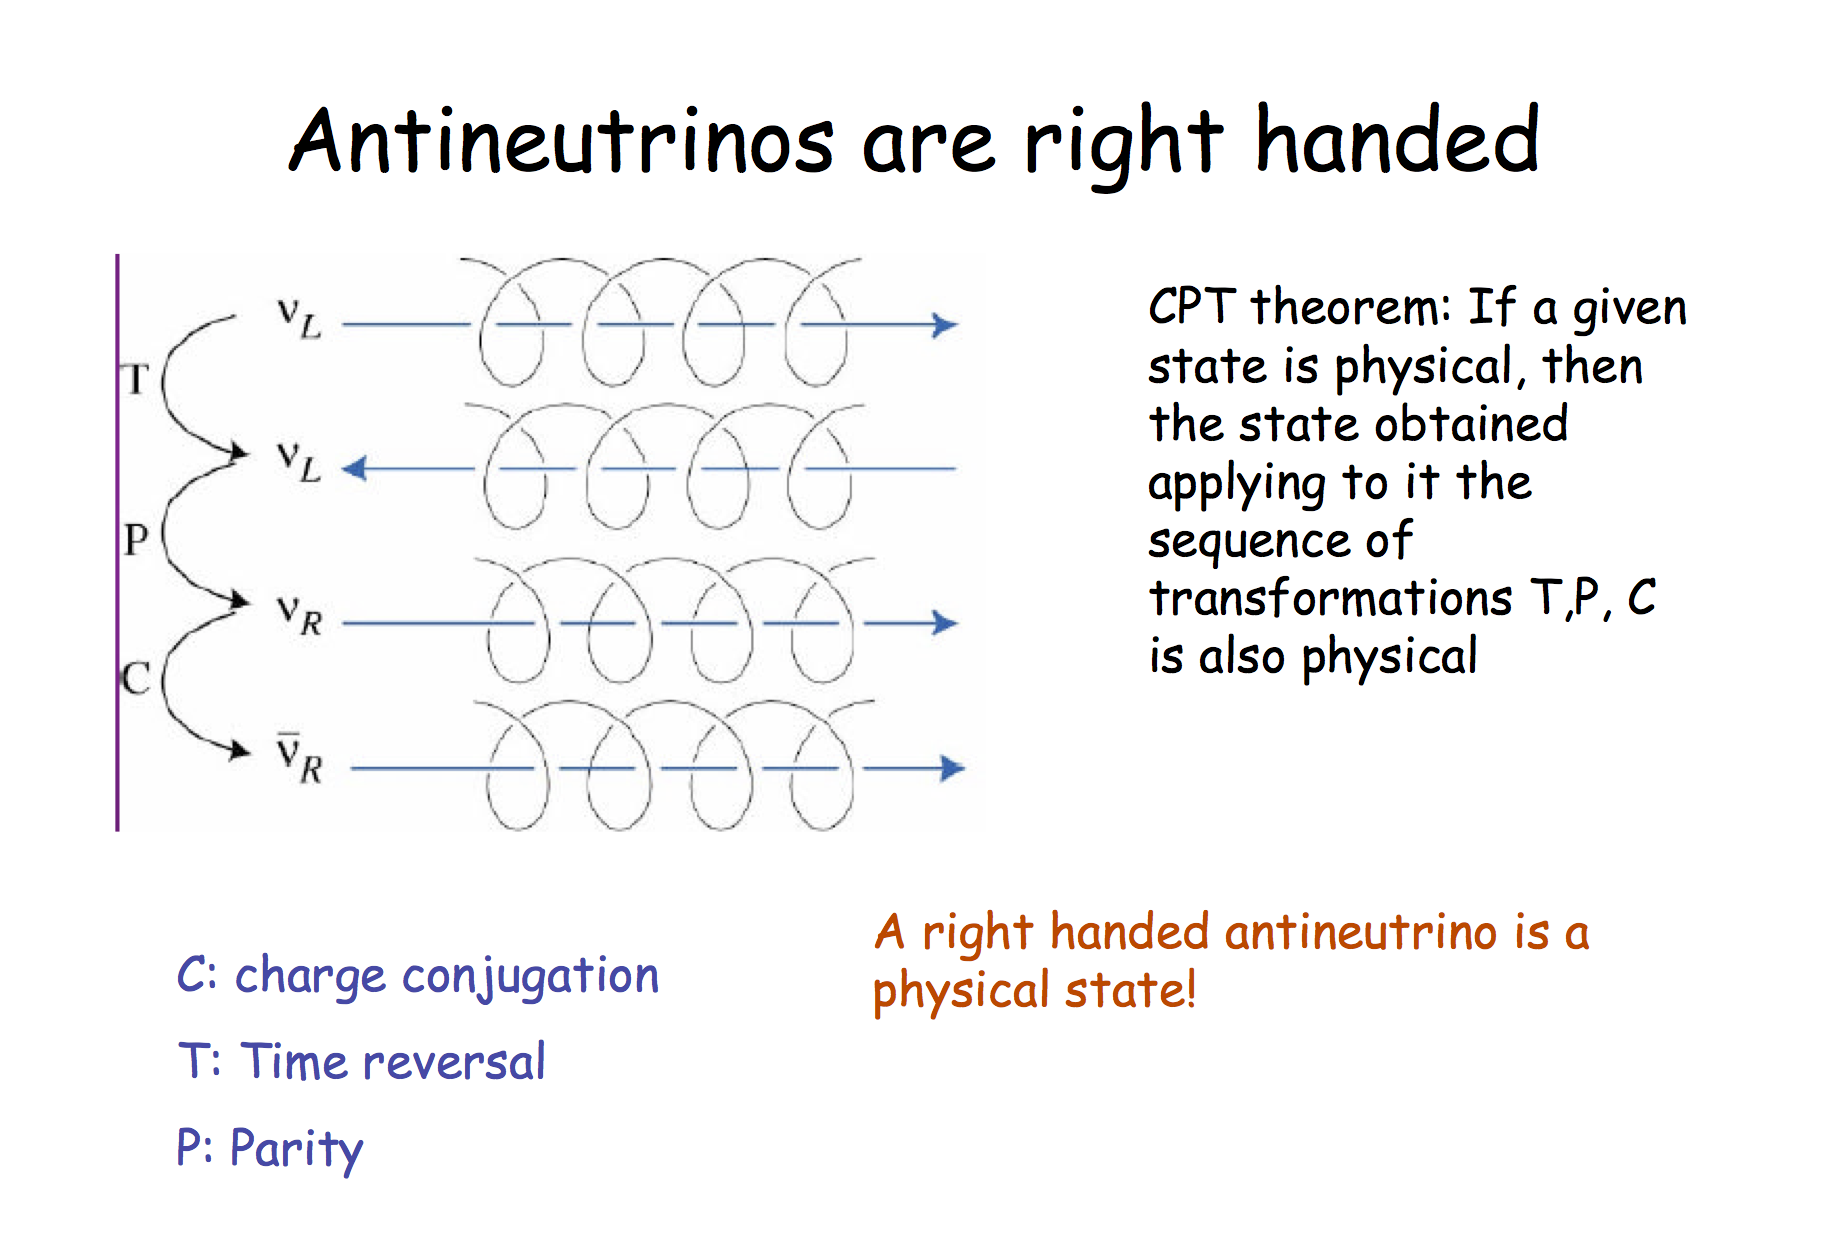
\includegraphics[scale=0.35]{AntineutrinosRH.png}
%
%\end{frame}

%\begin{frame}
%\frametitle{What do we talk about when we talk about (Standard Model) neutrinos?}
%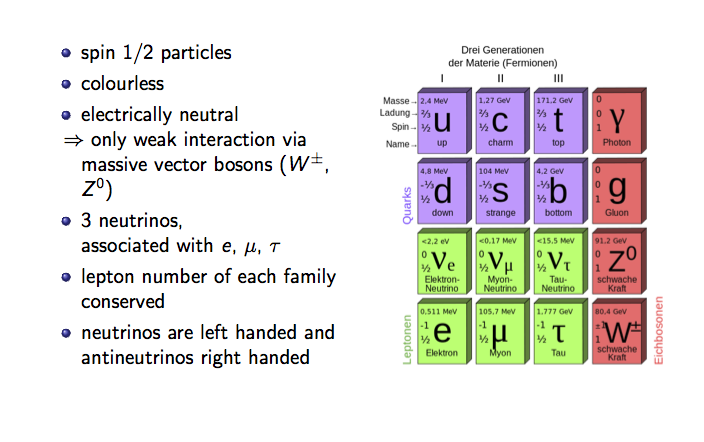
\includegraphics[scale=0.90]{NeutrinoOverview.png}
%\end{frame}

\begin{frame}
\frametitle{Neutrinos through the looking glass}
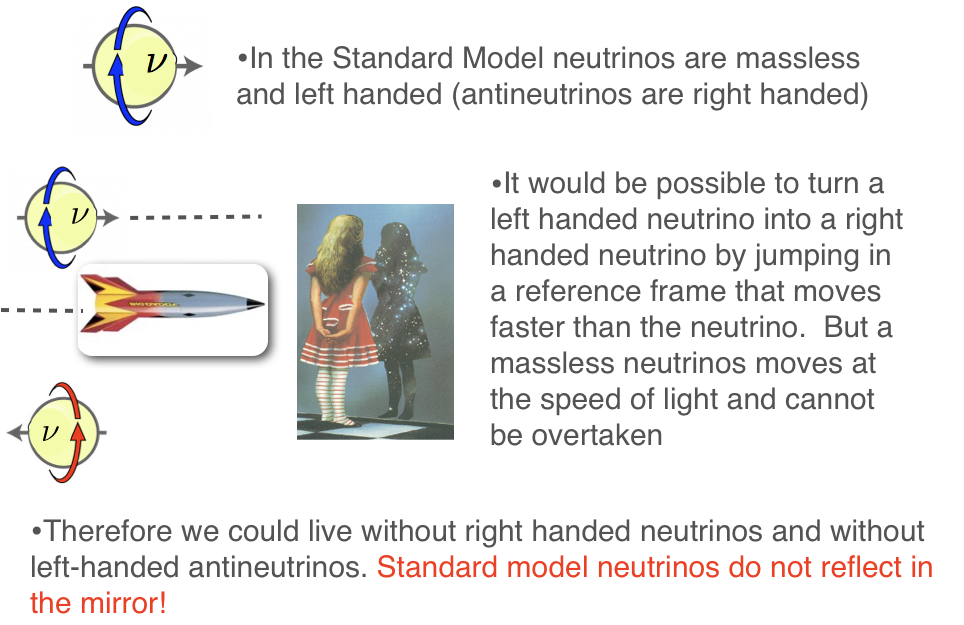
\includegraphics[scale=0.33]{img/NeutrinosLookingG.png}
\end{frame}

\begin{frame}
\frametitle{But what if neutrinos are massive}
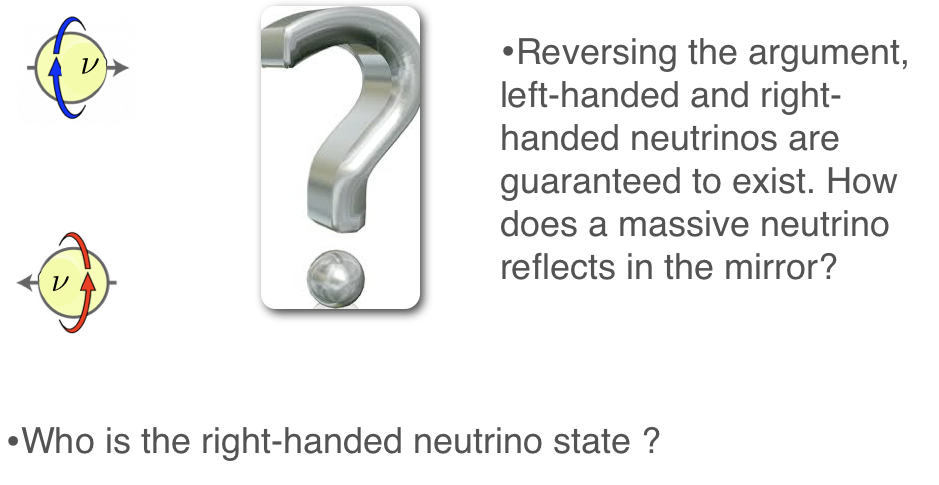
\includegraphics[scale=0.33]{img/WhatIfNeutrinoMassive.png}

\end{frame}






\section{Massive neutrinos}
%\begin{frame}
%\frametitle{Massless particles and helicity}
%\begin{columns}
%\column{0.5\textwidth}
%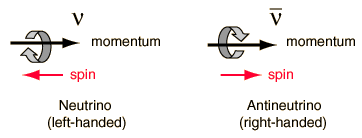
\includegraphics[scale=0.35]{img/NeutrinoHelicity.png}
%
%Helicity is the spin projection in the direction of motion.
%\[
%h = \frac{\va{\sigma}\cdot \va{p}}{p}
%\]
%In the limit of $m \rightarrow 0$~ Dirac's equation(s) decouple in 
%two states with definite helicity:
% \begin{empheq}[box=\fbox]{align}
%(E +  \va{p}\cdot\va{\sigma}) \chi  & = 0 \nonumber \\
%(E -  \va{p}\cdot\va{\sigma}) \phi  & = 0 \nonumber
%\end{empheq}
%The particle has negative helicity and the antiparticle positive helicity. \alert{Massless particles have well defined helicity}. \column{0.5\textwidth}
%
%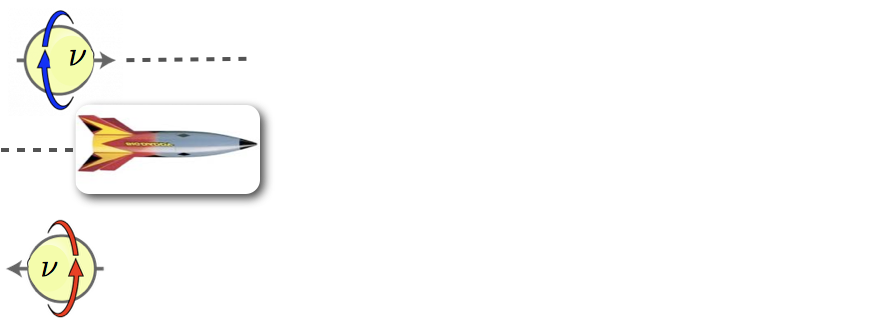
\includegraphics[scale=0.30]{img/neutrinoBoost2.png}
%
%For massive particles, helicity depends on the reference frame. One can always jump into a reference system faster than that of the particle and see its helicity flip.
%
%But massless particles travel at the speed of light and cannot be overtaken. The helicity becomes a constant of motion. 
%\end{columns}
%
%\end{frame}
%
%\begin{frame}
%\frametitle{Neutrino oscillations}
%%\begin{columns}
%%\column{0.4\textwidth}
%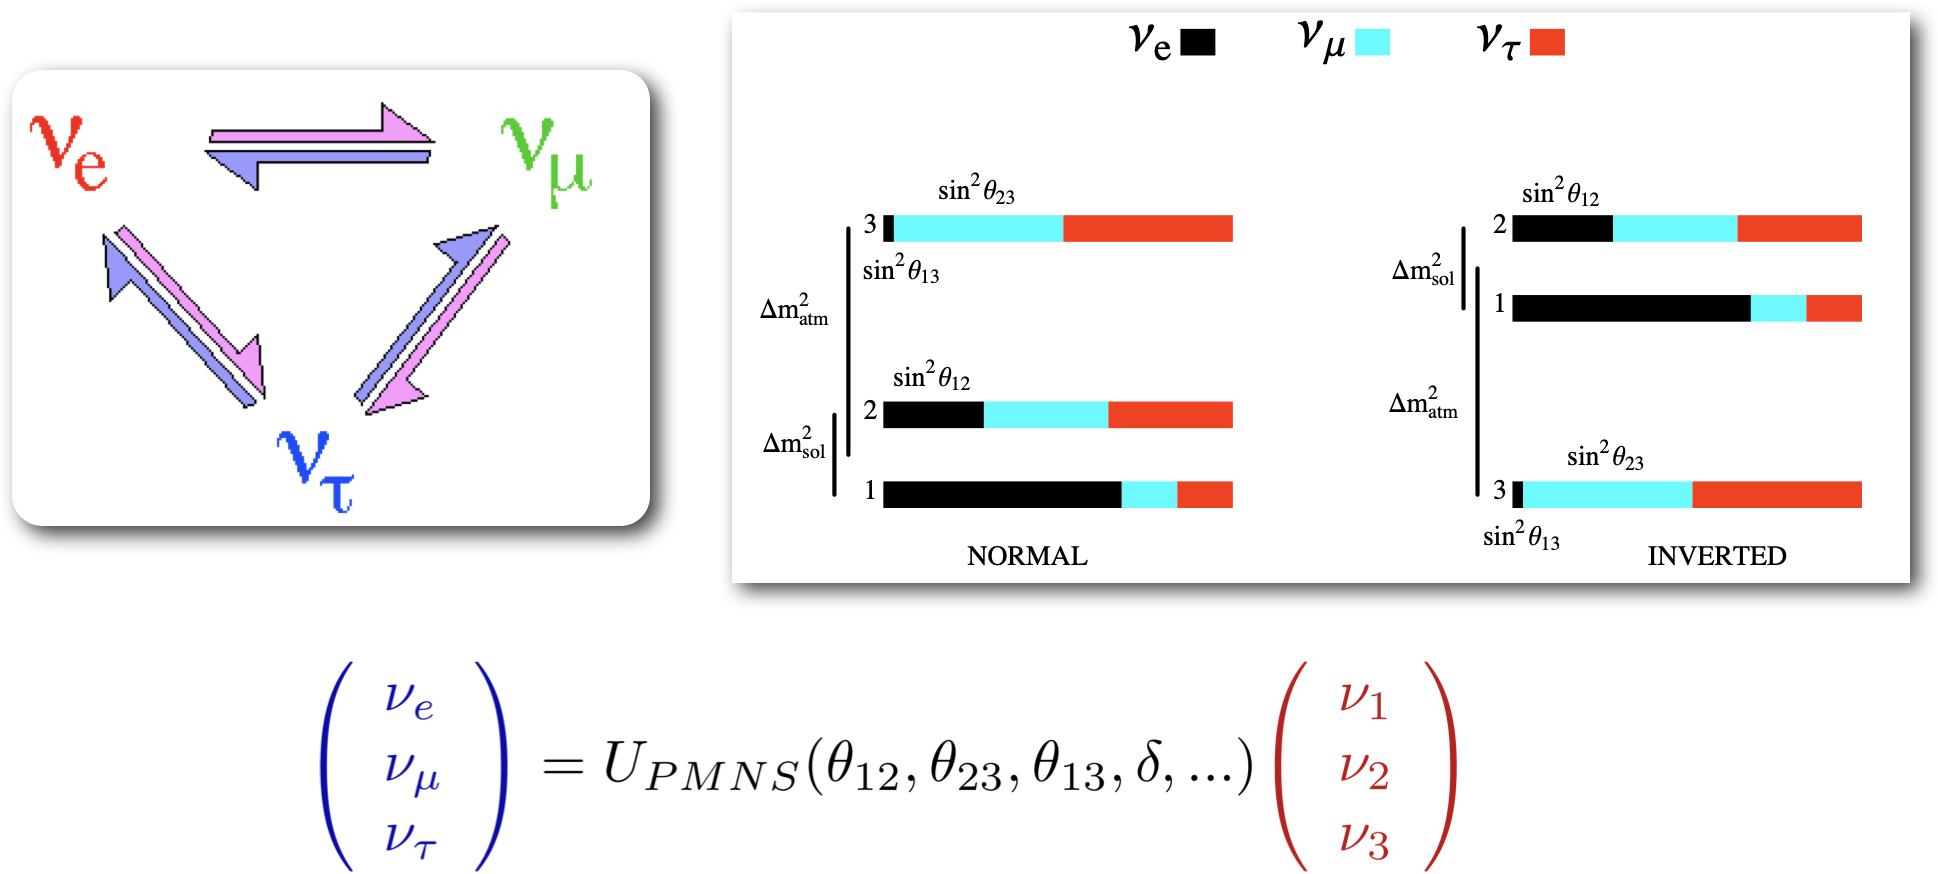
\includegraphics[scale=0.30]{img/neutrinoOscillations.png}
%%\column{0.4\textwidth}
%%\begin{block}{}
%
%Neutrino oscillation experiments (a story to be told some other time) have established that neutrinos are massive. Their mass is, however, very small. This is the reason why parity experiments found the neutrino to be left handed, since the effects associated to their masses are of the order of $m/E$~where $m$~is the mass of the neutrino (tiny) and $E$~the energy of the process (much larger). 
%
%\alert{But how do we give a mass to the neutrinos?} 
%
%%\end{block}
%%\end{columns}
%\end{frame}
%
%\begin{frame}
%\frametitle{Electron mass}
%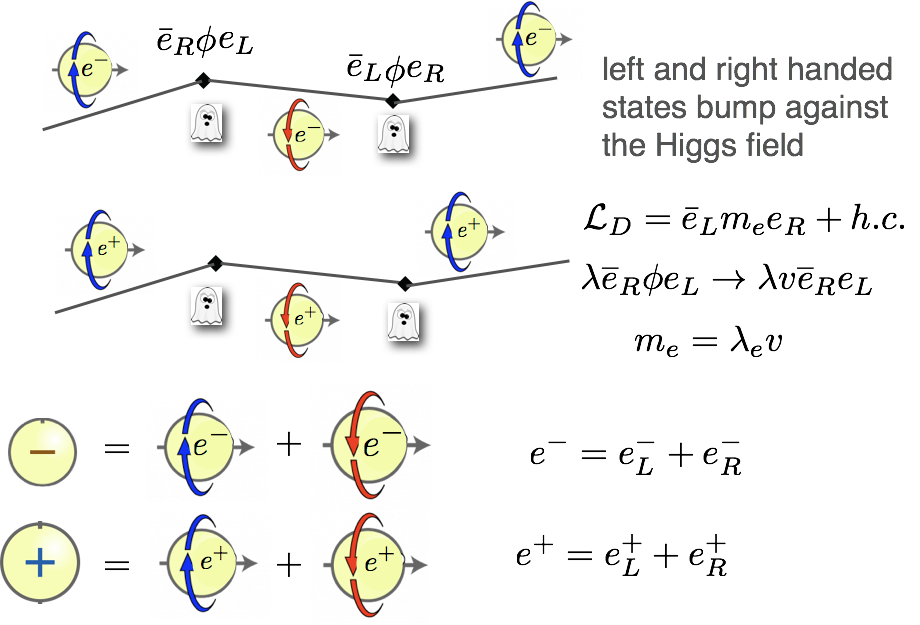
\includegraphics[scale=0.30]{img/ElectronMass.png}
%\end{frame}

\begin{frame}
\frametitle{Neutrino mass (Dirac recipe)}
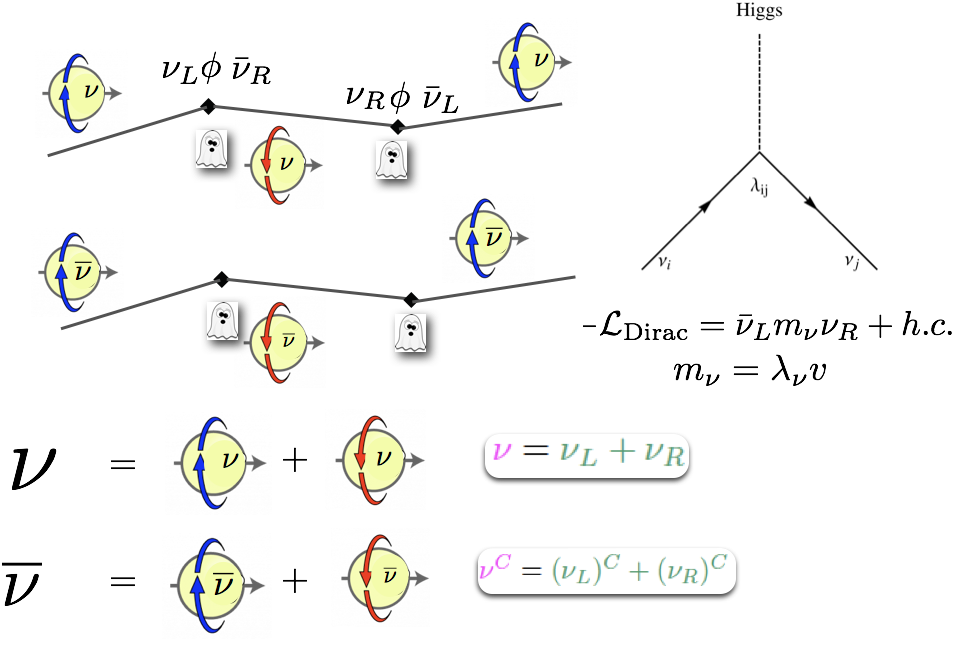
\includegraphics[scale=0.30]{img/NeutrinoMassDirac.png}
\end{frame}

\begin{frame}
\frametitle{Deus ex machina}
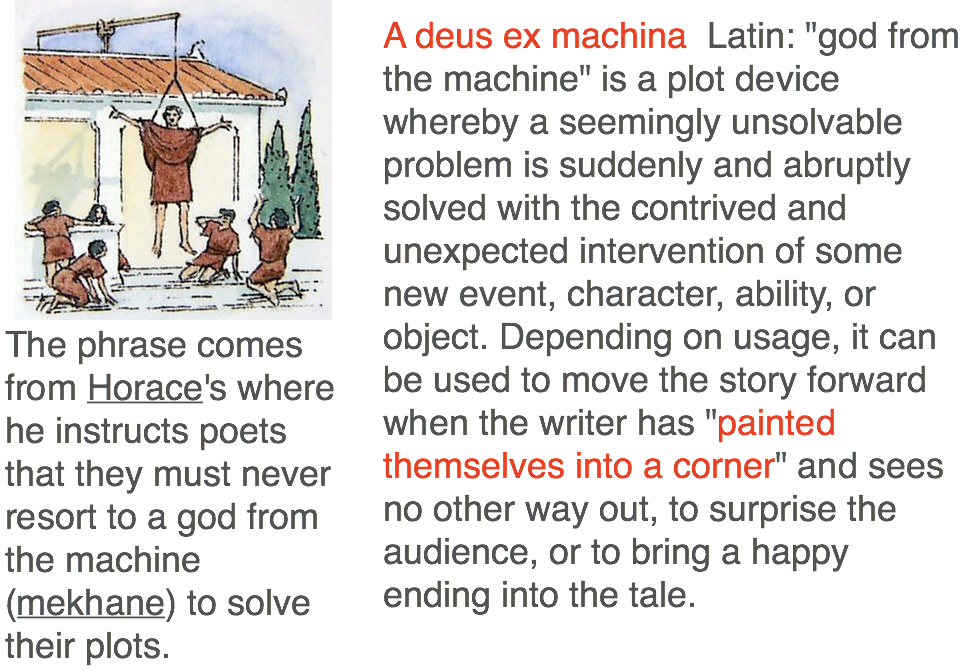
\includegraphics[scale=0.30]{img/DeusExMachina.png}
\end{frame}

\begin{frame}
\frametitle{Dirac neutrino mass: Deus ex machina}
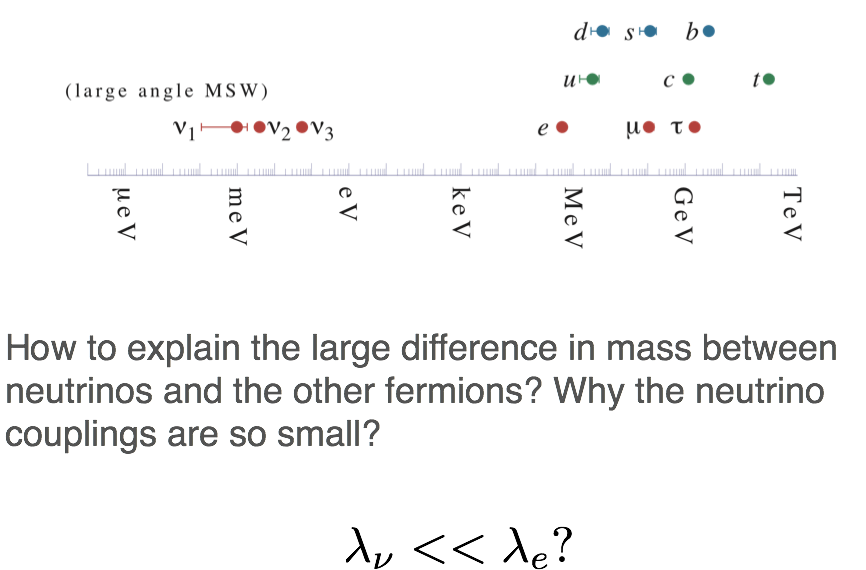
\includegraphics[scale=0.30]{img/SmallNeutrinoMasses.png}
\end{frame}

\begin{frame}
\frametitle{Majorana neutrinos}
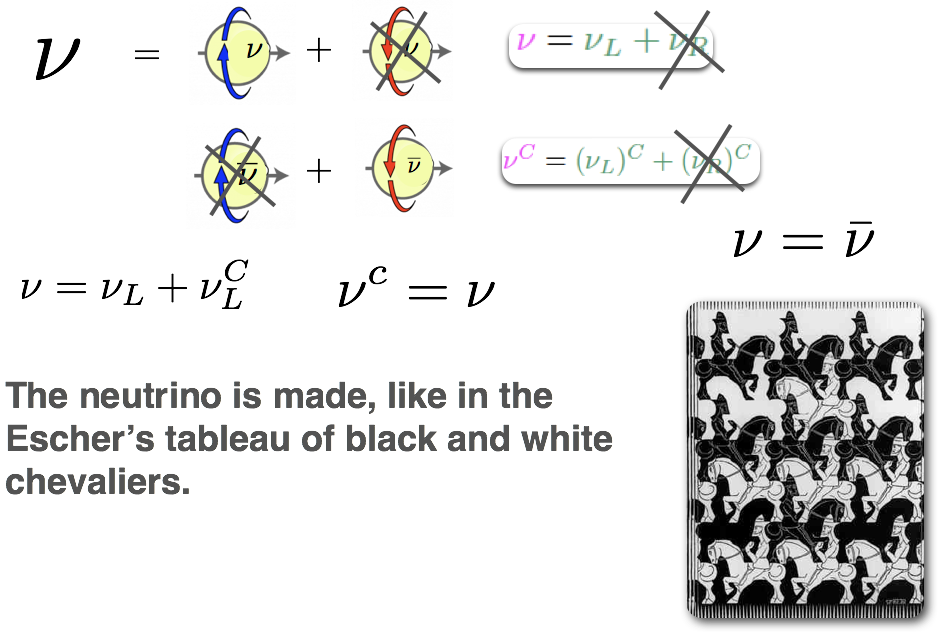
\includegraphics[scale=0.30]{img/MajoranaNeutrinosCartoon.png}
\end{frame}

\begin{frame}
\frametitle{Majorana mass}
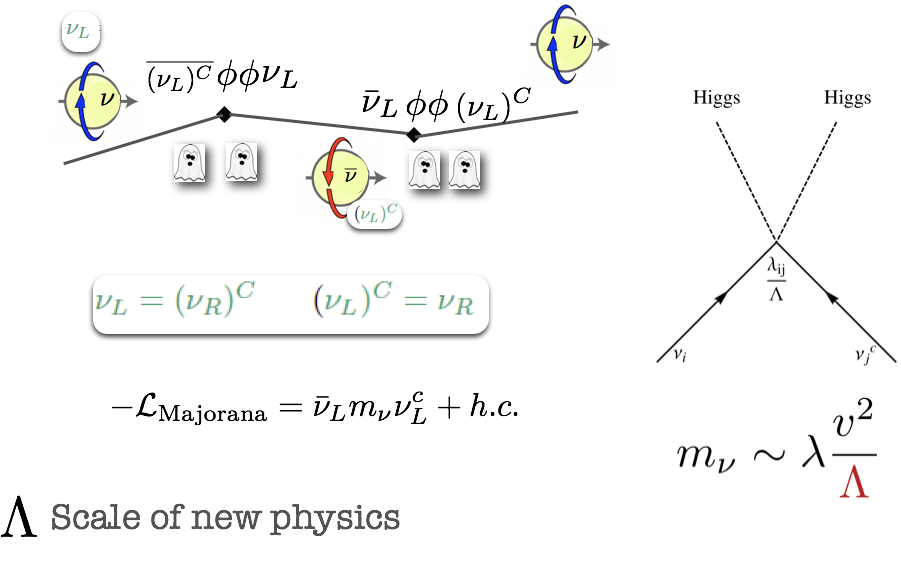
\includegraphics[scale=0.30]{img/MajoranaMass.png}
\end{frame}

\begin{frame}
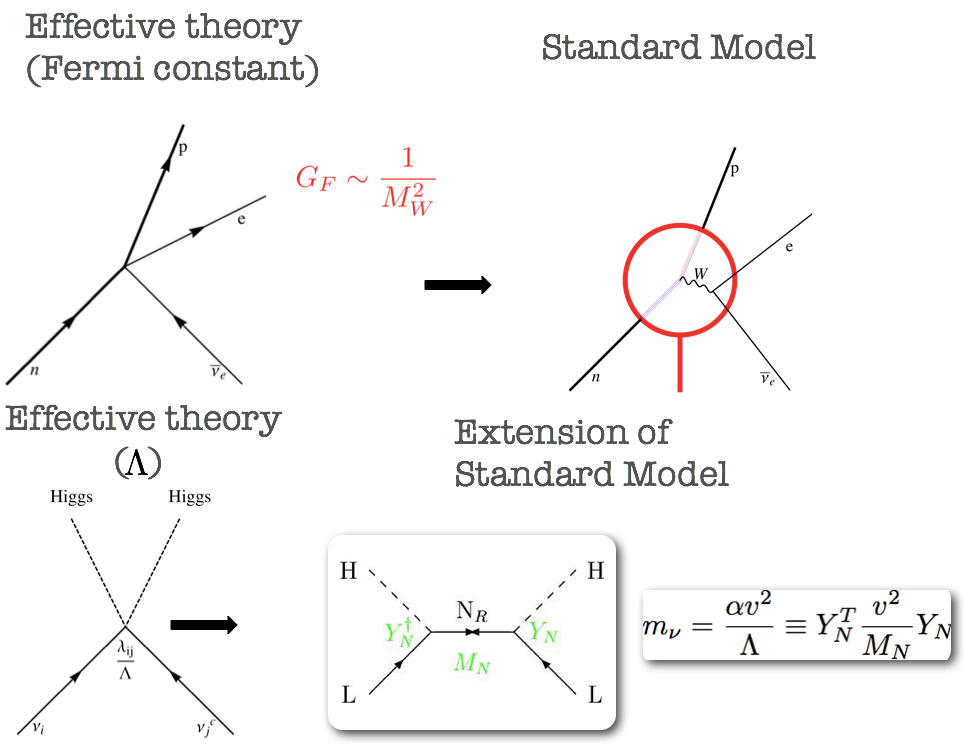
\includegraphics[scale=0.30]{img/Effective.png}
\end{frame}

\begin{frame}
\frametitle{The mystery of the missing antimatter}
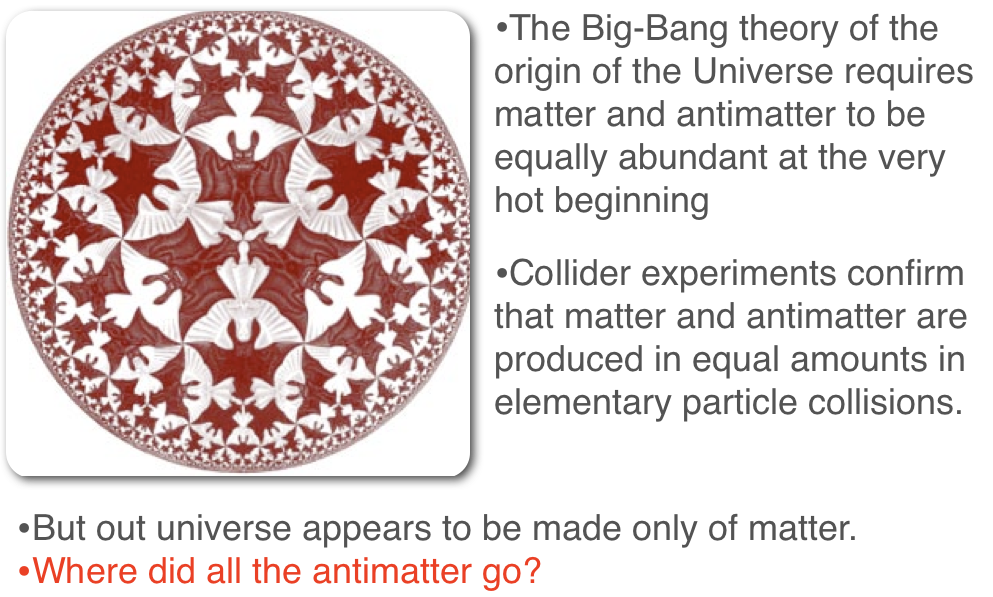
\includegraphics[scale=0.30]{img/MissingAntiMatter.png}
\end{frame}

\begin{frame}
\frametitle{CP violation and Majorana neutrinos}
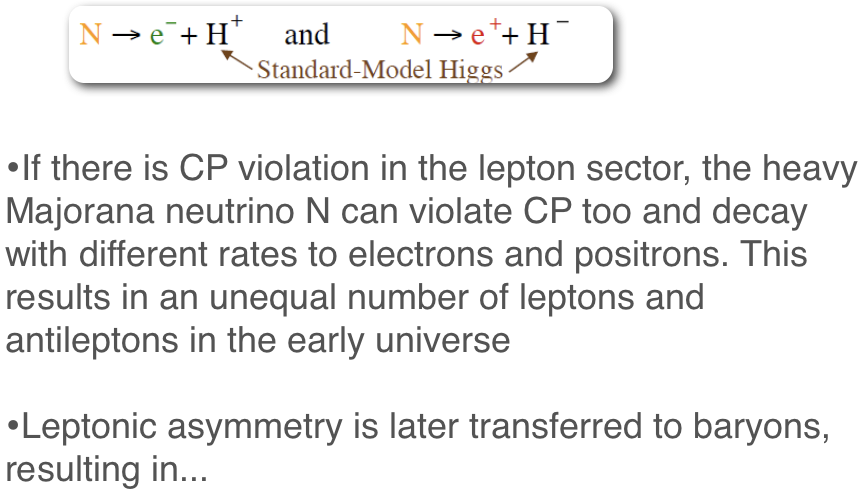
\includegraphics[scale=0.30]{img/CP.png}
\end{frame}

\begin{frame}
\frametitle{We are the leftovers}
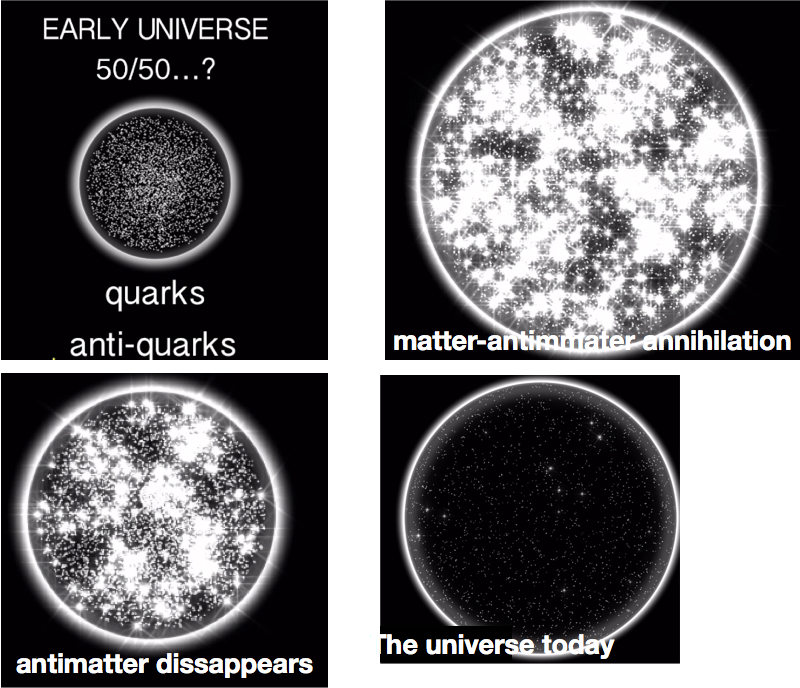
\includegraphics[scale=0.30]{img/MissingUniverse.png}
\end{frame}
%

\begin{frame}
\frametitle{A formula for the Universe}
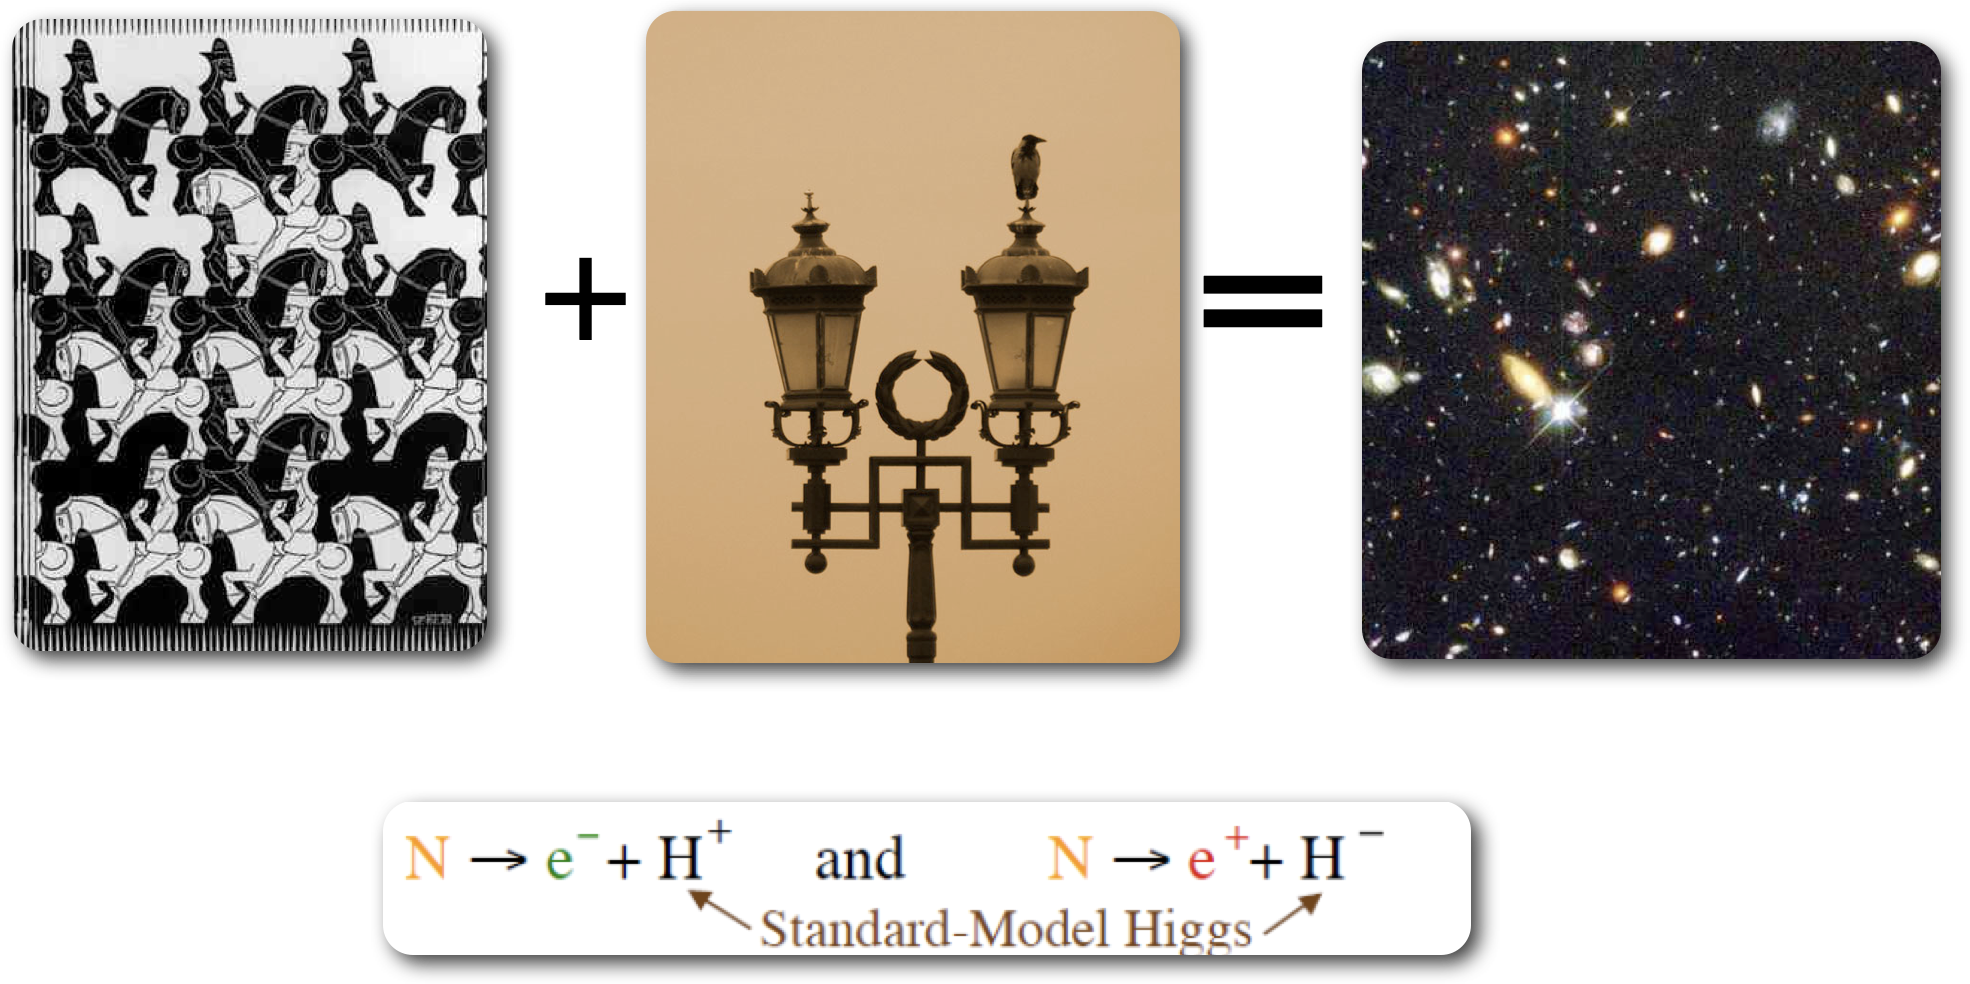
\includegraphics[scale=0.30]{img/formulaUniverse.png}
\end{frame}











\section{Double or Nothing}
\begin{frame}
\frametitle{Are neutrinos Majorana Particles?}

\includegraphics[scale=0.30]{img/DoubleOrNothing.png}
\end{frame}

\begin{frame}
\frametitle{Double Beta Decay}
\begin{columns}
\column{0.45\textwidth}
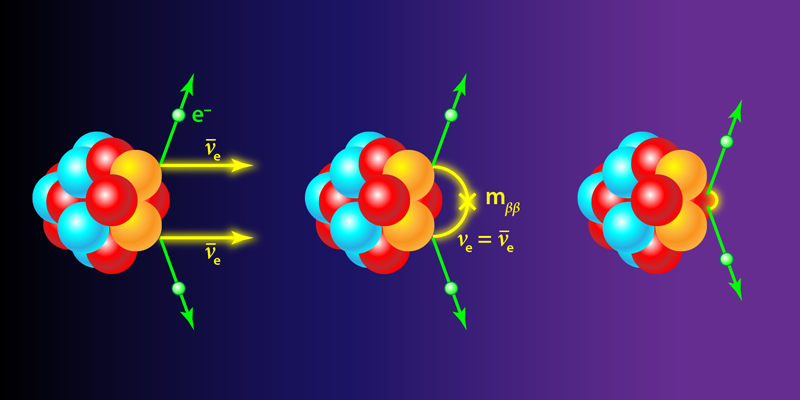
\includegraphics[scale=0.2]{img/doublebeta.png}
 
 \column{0.5\textwidth}
%\begin{block}{}
Double Beta ($\beta\beta$) decay occurs in a number of nuclear isotopes. 

The allowed process ($\beta\beta 2\nu$) is ``simply" the simultaneous decay of two neutrons. It is a very rare (long lifetime), but otherwise totally standard reaction. The lifetime of the process depends on the isotope, the order of magnitude is $10^{18}-10^{20}$ years (compare with the lifetime of the Universe, $10^{10}$ years.

The ``forbidden process" (($\beta\beta 0\nu$) occurs if and only if neutrinos are Majorana particles. The lifetime of the process depends of the neutrino masses and mixing angles. Experimentally we know that $T_0 > 10^{26}$ years. Current data suggests that $T_0 > 10^{27}$ years at least, quite likely larger. 
%\end{block}
\end{columns}
\end{frame}

\begin{frame}
\frametitle{Double Beta Decay isotopes}
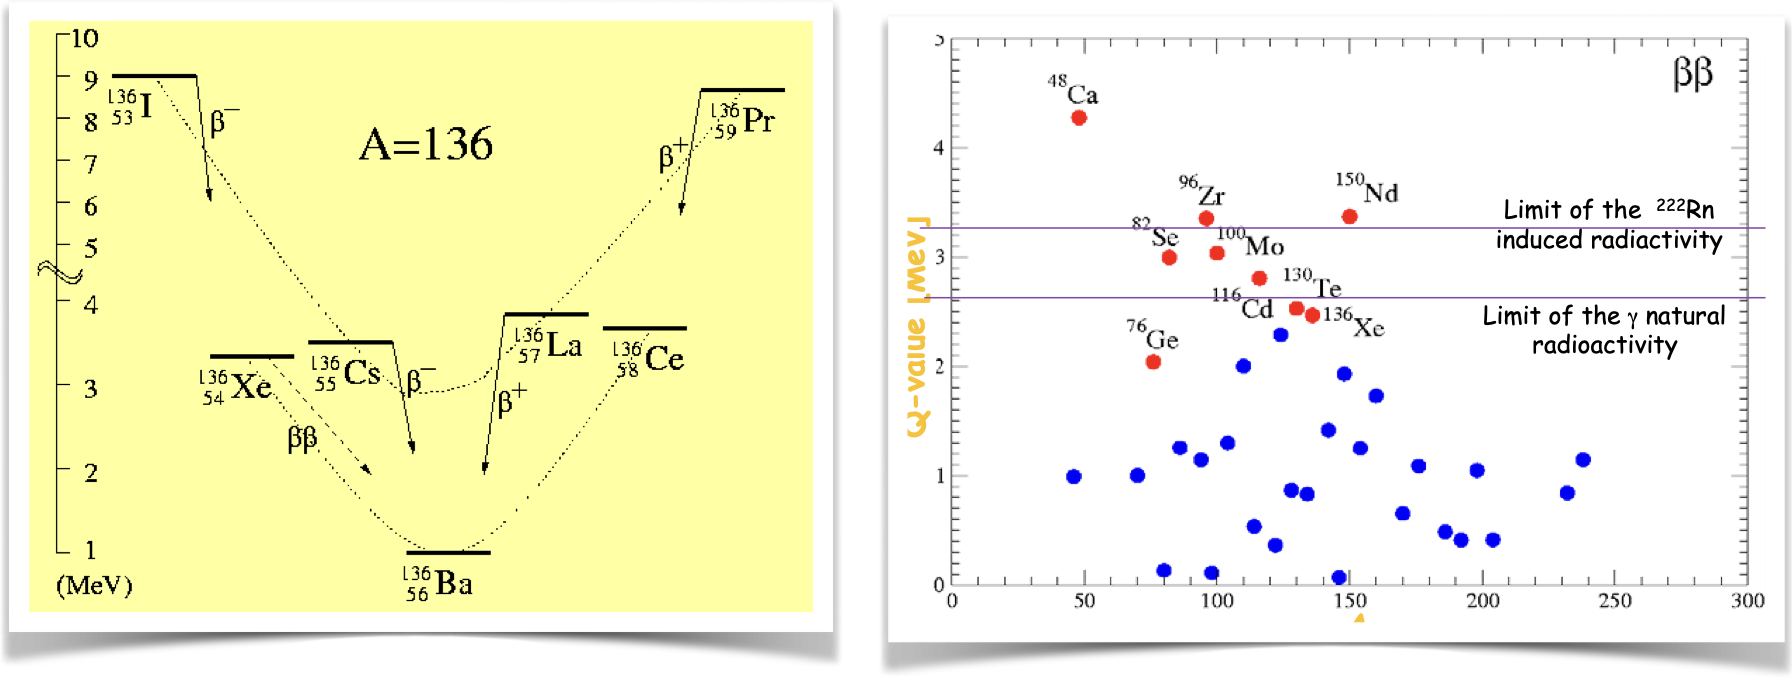
\includegraphics[scale=0.35]{img/BBIsotopes.png}
\end{frame}

\begin{frame}
\frametitle{Feynman Diagrams}
\begin{columns}
\column{0.45\textwidth}
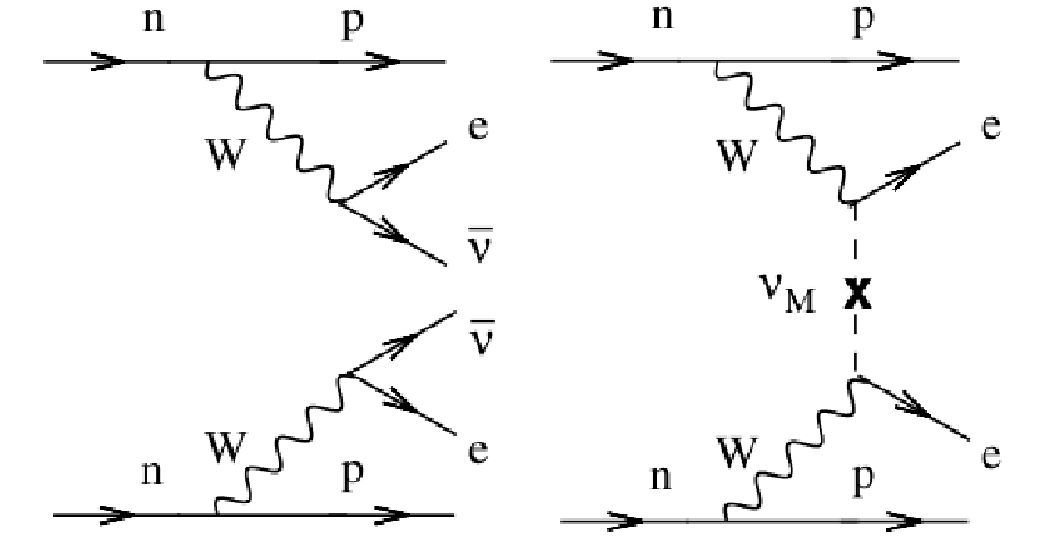
\includegraphics[scale=0.15]{img/feynman2.png}
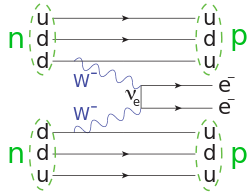
\includegraphics[scale=0.35]{img/250px-Double_beta_decay_feynman.svg.png}
 
 \column{0.5\textwidth}
%\begin{block}{}
The first diagram shows two independent neutrons emitting a W (which turns them into protons). The W, in turn, couples to and electron and a neutrino. This is simply the standard double beta decay, with a much smaller probability dictated by the fact that the two neutrons must decay simultaneously.  

The second diagram shows an alternative decay route. Here, the two W are connected by a neutrino. This requires two conditions: a) the neutrino is virtual (like the W), and b) the neutrino helicity flips between emission and absorption, so that one W emits an antineutrino and the other W absorbs a neutrino. This can only happen if the neutrino is a Majorana Particle. 
%\end{block}
\end{columns}
\end{frame}


\begin{frame}
\frametitle{A formula for $\beta\beta 0 \nu$ lifetime}

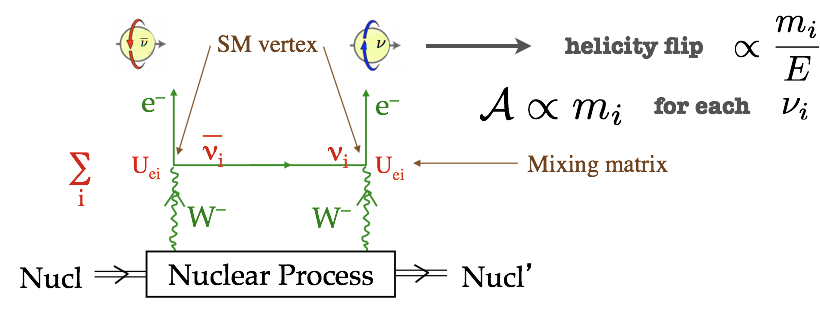
\includegraphics[scale=0.35]{img/DoubleBetaDiagram2.png}

%\begin{block}


\begin{empheq}[box=\fbox]{align}
  (T_{1/2}^{0\nu})^{-1} = G^{0\nu} |M^{0\nu}|^2 m_{\beta\beta}^2 \nonumber
\end{empheq}
%\end{block}
\end{frame}



%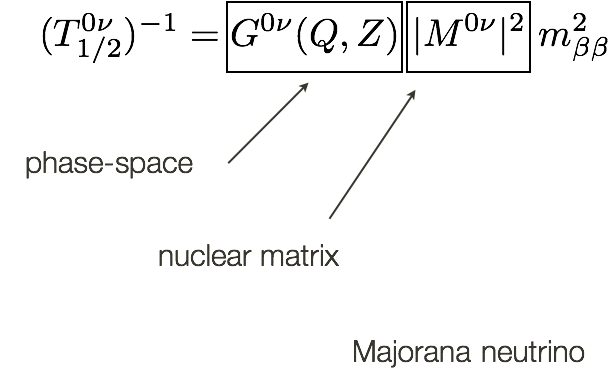
\includegraphics[scale=0.30]{DoubleBetaLifetime.png}
%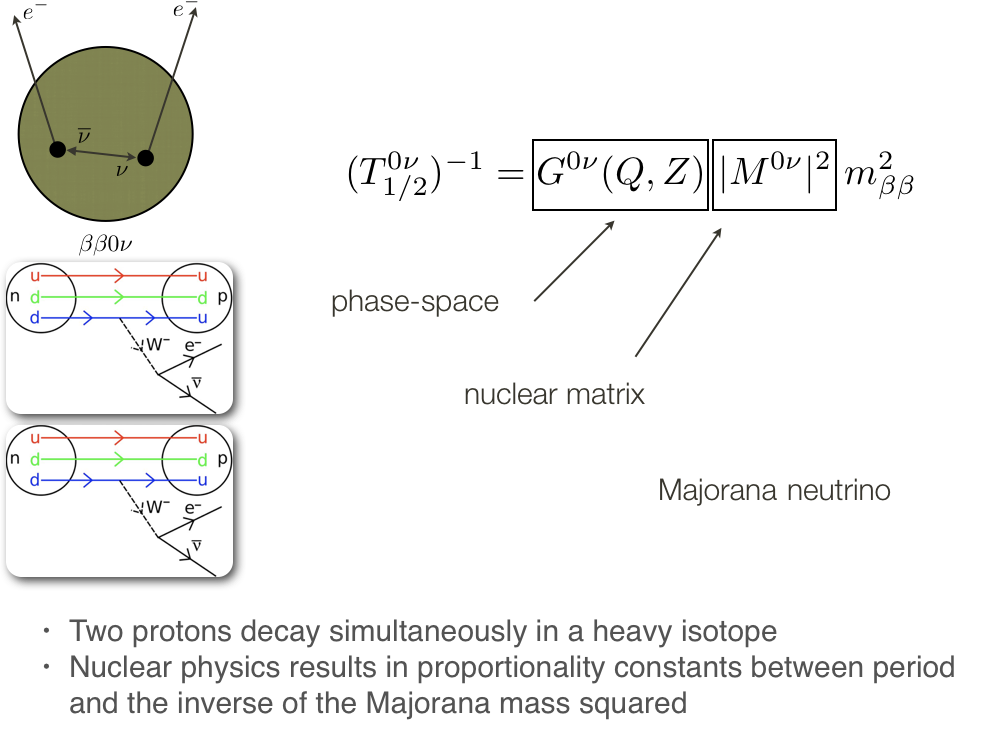
\includegraphics[scale=0.20]{img/bbmatrix.png}

\begin{frame}
\frametitle{Majorana's Lanscape}
\begin{columns}
\column{0.55\textwidth}
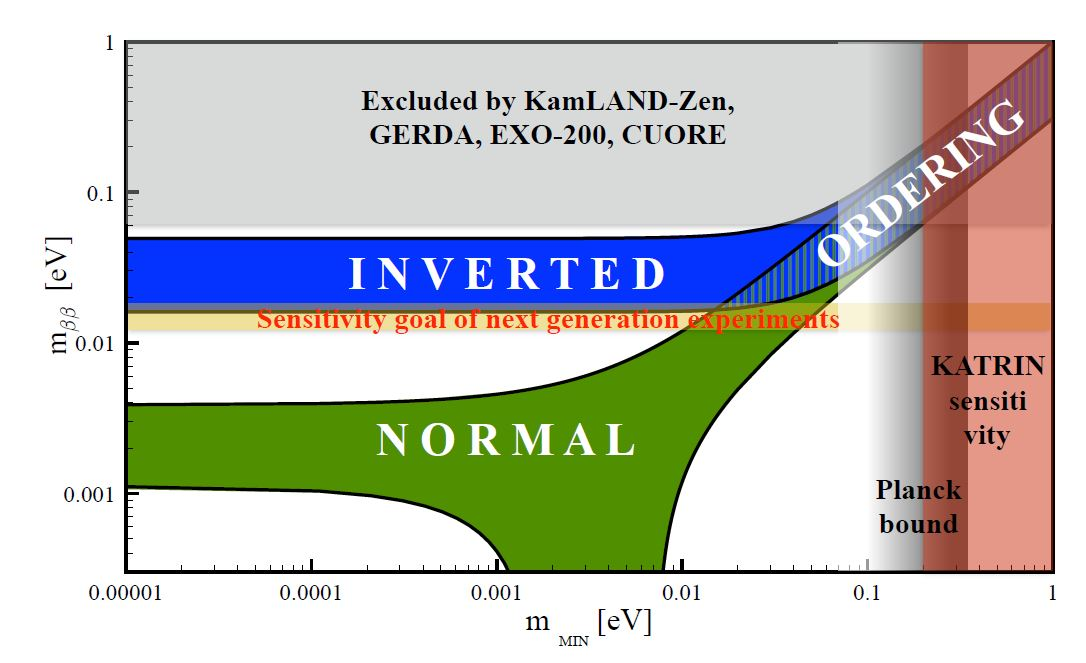
\includegraphics[scale=0.35]{img/doublebetas.jpg}
$T_{1/2}^{0\nu} \sim 10^{27}$y  $\approx m_{\beta\beta} \sim 20$meV. \alert{Explore IO}

 \column{0.45\textwidth}
\includegraphics[scale=0.25]{img/nuhierarchies.png}
$T_{1/2}^{0\nu} \sim 10^{29}$y  $\approx m_{\beta\beta} \sim 2$meV. \alert{Explore NO}
\end{columns}


\end{frame}



\begin{frame}
\frametitle{An ideal double beta decay experiment}
\begin{columns}
\column{0.45\textwidth}
\includegraphics[scale=0.35]{img/IdealBB2.png}
\column{0.5\textwidth}
%\begin{block}{}
$\bullet$~Get yourself a detector with perfect energy resolution.

$\bullet$~Measure the energy of the emitted electrons and select those with $(T_1+T_2)/Q = 1$.

$\bullet$~Count the number of events and calculate the corresponding half-life. 

$\bullet$~In ${136}^{}Xe$, a perfect detector of 1 ton observes 3 events for a lifetime of $10^{27}$ y ($\sim$ 20 meV).

$\bullet$~Improvement in sensitivity to $m_{\beta\beta}$ goes with $\sqrt{T}$ ($\beta\beta$ tragedy number one) 
%\end{block}
\end{columns}
\end{frame}


\begin{frame}
\frametitle{Why $\beta\beta0\nu$ experiments are difficult}
\begin{columns}
\column{0.45\textwidth}
\includegraphics[scale=0.35]{img/Uchain.png}
\column{0.5\textwidth}
$\bullet$~Earth is a very radioactive planet. There are about 3 grams o ${238}^{}U$ and 9 grams of ${232}^{}Th$ per ton of rock around us.

$\bullet$~This is an intrinsic activity of the order of 60 Bq/kg of ${238}^{}U$ and  90 Bq/kg of ${232}^{}Th$.

$\bullet$~The lifetime of ${238}^{}U$ is of the order of $10^9$ y and that of ${232}^{}Th \sim 10^{10}$ y. 

$\bullet$~We want to explore lifetimes of of the order of $10^{27} -10^{29}$ y.

$\bullet$~The problem is much harder than finding a needle in a haystack 
\end{columns}
\end{frame}

\begin{frame}
\frametitle{Majorana's Beach}
\includegraphics[scale=0.30]{img/beach}

$\bullet$~Majorana’s beach: A beach with $10^{17}$ grains of sand.

$\bullet$~About $1.5 \times 10^9$ grains per square meter (to a depth of 3 m).

$\bullet$ Thus, Majorana’s beach is 70 km long and 1 km wide.

$\bullet$~Next generation $\beta\beta 0 \nu$ experiments will try to find a grain of sand in such a beach. 
\end{frame}

\begin{frame}
\frametitle{The signal and the noise}
\includegraphics[scale=0.30]{img/signalAndNoise.png}
\end{frame}


\begin{frame}
\frametitle{Recipe for a $\beta \beta 0 \nu$ experiment}
\includegraphics[scale=0.30]{img/RecipeExperiment.png}
\end{frame}


%
%
%
%
%


\section{To see a World in a Grain of Sand }

\begin{frame}
\frametitle{Every odyssey starts with a terrific idea}
\includegraphics[scale=0.30]{img/nextTroy.png}
\end{frame}

\begin{frame}
\frametitle{And utter ignorance of the upcoming complications}
\includegraphics[scale=0.30]{img/bbAndTroy.png}
\end{frame}

\begin{frame}
\frametitle{From dream to reality...}
\includegraphics[scale=0.30]{img/nextCollague.png}
\end{frame}

\begin{frame}
\frametitle{NEXT detector concept}
\includegraphics[scale=0.30]{img/PrincipleNext2.png}
\end{frame}

\begin{frame}
\frametitle{From an empty space}
\includegraphics[scale=0.30]{img/emptyLSC.png}
\end{frame}

\begin{frame}
\frametitle{To a busy place}
\includegraphics[scale=0.25]{img/lsc2021.png}
\end{frame}

\begin{frame}
\frametitle{Technology works}
\includegraphics[scale=0.20]{img/whiteResults.png}
\end{frame}

\begin{frame}
\frametitle{But no signal}
\includegraphics[scale=1.00]{img/nosignal.jpg}
\end{frame}

\begin{frame}
\frametitle{From reality to dream}
\includegraphics[scale=0.20]{img/nextProgram.png}
\end{frame}


\begin{frame}
\frametitle{BOLDly go where no one has bone before...}
\begin{columns}
\column{0.45\textwidth}
\includegraphics[scale=0.09]{img/enterprise.jpg}
\column{0.5\textwidth}
$\bullet$~To explore lifetimes of $10^{27}$ y we need an exposure of the order of 1 ton$\cdot$year.

$\bullet$~Thus $10^{28}$ y could be reached achieving exposures of the order of 10 ton$\cdot$year. It could even be that $10^{28}$ y is conceivable. 

$\bullet$~However, this is only possible if we achieve a \alert{fully background free experiment}

$\bullet$~This is the goal of the BOLD project (ERC/Synergy grant, 2020). 

\end{columns}
\end{frame}

\begin{frame}
\frametitle{A new skin for the old ceremony}
\begin{columns}
\column{0.45\textwidth}
\includegraphics[scale=0.2]{img/bariumTagging.png}
\column{0.5\textwidth}
$\bullet$~All current (and planned) $\beta \beta 0 \nu$ experiments detect only the electromagnetic part of the decay (e.g., the electrons). 

$\bullet$~NEXT-BOLD proposed to detect both the electrons and the $Ba^{2+}$ dication. 
 
$\bullet$~Radioactivity produces electrons but not isolated $Ba^{2+}$ dications. 

$\bullet$~But most importantly, we will detect the signal in (delayed) coincidence. \alert{Some trick that allowed the discovery of the neutrino}

\end{columns}
\end{frame}

\begin{frame}
\frametitle{BOLD ingredients}
\begin{columns}
\column{0.45\textwidth}
\includegraphics[scale=0.15]{img/FBI.png}

$\bullet$~Idea (Dave Nygren): Exploit single molecule fluorescent imaging (SFMF) to visualise (“tag”) a  single  $Ba^{2+}$ dication as it arrives at the TPC cathode.

$\bullet$~Fluorescent Bicolor $Ba^{2+}$ sensor (Fernando Coss\'io):Able to trap ("chelate") the dication and change luminous response when this happens. 

\column{0.5\textwidth}
\includegraphics[scale=0.12]{img/nextBold.png}

$\bullet$~Bold Apparatus (JJGC): Capable to detect in delayed coincidence the electron signal (in anode) and the cation signal in cathode.


\end{columns}
\end{frame}

\begin{frame}
\frametitle{A Blue Spark may signal where the grain of sand lies}
\includegraphics[scale=0.18]{img/BaTaResults.png}

\end{frame}


\begin{frame}
\frametitle{Majorana Beach}
\includegraphics[scale=0.30]{img/MajoranaBeach2.png}
\end{frame}
%
%





%\input{lsc/diracRevisited.tex}
%%\begin{frame}
%\frametitle{Massless particles and helicity}
%\begin{columns}
%\column{0.5\textwidth}
%\includegraphics[scale=0.35]{img/NeutrinoHelicity.png}
%
%Helicity is the spin projection in the direction of motion.
%\[
%h = \frac{\va{\sigma}\cdot \va{p}}{p}
%\]
%In the limit of $m \rightarrow 0$~ Dirac's equation(s) decouple in 
%two states with definite helicity:
% \begin{empheq}[box=\fbox]{align}
%(E +  \va{p}\cdot\va{\sigma}) \chi  & = 0 \nonumber \\
%(E -  \va{p}\cdot\va{\sigma}) \phi  & = 0 \nonumber
%\end{empheq}
%The particle has negative helicity and the antiparticle positive helicity. \alert{Massless particles have well defined helicity}. \column{0.5\textwidth}
%
%\includegraphics[scale=0.30]{img/neutrinoBoost2.png}
%
%For massive particles, helicity depends on the reference frame. One can always jump into a reference system faster than that of the particle and see its helicity flip.
%
%But massless particles travel at the speed of light and cannot be overtaken. The helicity becomes a constant of motion. 
%\end{columns}
%
%\end{frame}
%
%\begin{frame}
%\frametitle{Neutrino oscillations}
%%\begin{columns}
%%\column{0.4\textwidth}
%\includegraphics[scale=0.30]{img/neutrinoOscillations.png}
%%\column{0.4\textwidth}
%%\begin{block}{}
%
%Neutrino oscillation experiments (a story to be told some other time) have established that neutrinos are massive. Their mass is, however, very small. This is the reason why parity experiments found the neutrino to be left handed, since the effects associated to their masses are of the order of $m/E$~where $m$~is the mass of the neutrino (tiny) and $E$~the energy of the process (much larger). 
%
%\alert{But how do we give a mass to the neutrinos?} 
%
%%\end{block}
%%\end{columns}
%\end{frame}
%
%\begin{frame}
%\frametitle{Electron mass}
%\includegraphics[scale=0.30]{img/ElectronMass.png}
%\end{frame}

\begin{frame}
\frametitle{Neutrino mass (Dirac recipe)}
\includegraphics[scale=0.30]{img/NeutrinoMassDirac.png}
\end{frame}

\begin{frame}
\frametitle{Deus ex machina}
\includegraphics[scale=0.30]{img/DeusExMachina.png}
\end{frame}

\begin{frame}
\frametitle{Dirac neutrino mass: Deus ex machina}
\includegraphics[scale=0.30]{img/SmallNeutrinoMasses.png}
\end{frame}

\begin{frame}
\frametitle{Majorana neutrinos}
\includegraphics[scale=0.30]{img/MajoranaNeutrinosCartoon.png}
\end{frame}

\begin{frame}
\frametitle{Majorana mass}
\includegraphics[scale=0.30]{img/MajoranaMass.png}
\end{frame}

\begin{frame}
\includegraphics[scale=0.30]{img/Effective.png}
\end{frame}

\begin{frame}
\frametitle{The mystery of the missing antimatter}
\includegraphics[scale=0.30]{img/MissingAntiMatter.png}
\end{frame}

\begin{frame}
\frametitle{CP violation and Majorana neutrinos}
\includegraphics[scale=0.30]{img/CP.png}
\end{frame}

\begin{frame}
\frametitle{We are the leftovers}
\includegraphics[scale=0.30]{img/MissingUniverse.png}
\end{frame}
%

\begin{frame}
\frametitle{A formula for the Universe}
\includegraphics[scale=0.30]{img/formulaUniverse.png}
\end{frame}











\end{document}